\documentclass{beamer}
%Information to be included in the title page:
\usetheme{Boadilla}
\definecolor{MITRed}{RGB}{163,31,52}
\definecolor{MITGray}{RGB}{138,139,140}
\usecolortheme[named=MITRed]{structure}

\setbeamertemplate{navigationsymbols}{}
\setbeamertemplate{headline}{\hfill
\includegraphics[width=1.5cm]{./MIT-logo-red-gray.png}\hspace{0.4cm}\vspace{-1.2cm}}
\beamertemplatenavigationsymbolsempty
\setbeamertemplate{blocks}[default]
\setbeamercolor{item projected}{bg=MITGray}
% \AtBeginSection[]
% {
% 	\begin{frame}
% 		\frametitle{Outline}
% 		\tableofcontents[currentsection]
% 	\end{frame}
% }
% \AtBeginSubsection[]
% {
% 	\begin{frame}
% 		\frametitle{Outline}
% 		\tableofcontents[currentsection,currentsubsection]
% 	\end{frame}
% }

\begin{document}
	\title[]{Industry, Committee, and Lobbying - Uncovering Congressional Stock Trading using Graph Data}
	% \subtitle{Johansson et al. (2016)}
	\author[Suyeol Yun]{Suyeol Yun}
	% \institute[MIT]{Massachusetts Institute of Technology}
	% \date{May 8, 2023}
	\frame{\titlepage}
	\section{Background}

	% \begin{frame}{Literature Review: Approaches \& Puzzles}
	% 	\begin{itemize}
	% 		% \item General Motivation: Electoral Accountability, Principal-Agent Problem, Conflicts of Interest, etc.
	% 		\item Initial focus: ``Excess return'' as an indicator of privileged knowledge usage in congressional stock trading
	% 		\item Ziobrowski (2004, 2011) discovers excess returns in both Senate and House stock trading
	% 		\item Eggers \& Hainmueller (2013): No excess returns found; Congress underperforms passive investments
	% 		\item A new puzzle emerges: Why are congressional investors underperforming?
	% 	\end{itemize}
	% 	% \centering	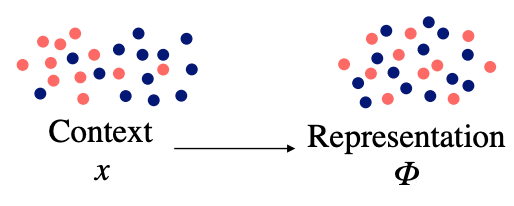
\includegraphics[scale=0.7]{./images/balancing.png}
	% \end{frame}

	\begin{frame}{Literature Review: Approaches \& Puzzles}
		\begin{itemize}
			\item Eggers \& Hainmueller (2014) examine congressional portfolios to determine disproportionate investments in firms with PAC contributions (+), district connections (+), or lobbying activities related to the congressperson's committee (-).
			\item \textit{``... We find no evidence that members disproportionately invest in companies to which they are connected through their committee assignments.''}
			\item This presents a new puzzle:

			- Extensive research exists on committee specialization (King, 1994; Asher et al., 1974; Myers, 2007)\\
			- Why is there an absence of a relationship between lobbying, committee assignments, and congressional investments?
		\end{itemize}
	\end{frame}

	\begin{frame}{Limitation of Eggers \& Hainmueller (2014)}
		$$w_{i j}=\alpha+\beta_1 \text { District }_{i j}+\beta_2 \text { Contributions }_{i j}+\beta_3 \text { Lobbying \& CA }_{i j}+\theta_i+\theta_j+\varepsilon_{i j}$$

		\begin{itemize}
			\item Firm-level analysis: $w_{ij}$ is portfolio weight of a firm $j$ for congressperson $i$ 
			\item Congresspeople invest at industry level
			\item Approximately 60\% of reported Senators' trades are ETFs or mutual funds, reflecting industry-level trading \\ 
				- e.g. Sheldon Whithouse traded US Medical Devices ETF (IHI)
			\item Lobbying involves complex industry-level interactions that a binary firm-level indicator and linear model cannot capture
		\end{itemize}
	\end{frame}

	\begin{frame}{Resolution: Using Graph Structured Data}
		\begin{itemize}
\item			Graphs are network data with nodes and edges
	\item		They capture intricate interactions among firms, bills, committees, and congresspersons
			\item Graph data compiled from Lobbyview, Senate/House Financial Disclosure, Congress, and naics.com
			\item url-based entity disambiguation; No more similarity based matching; $O(nm) \rightarrow O(n+m)$
		\item	The graph includes 55,700 nodes and 264,000 edges
			\item Data spans the 110th-117th Congresses (2007-2021)
		\end{itemize}
	\end{frame}

	\begin{frame}{Graph Data Specification}
		\centering	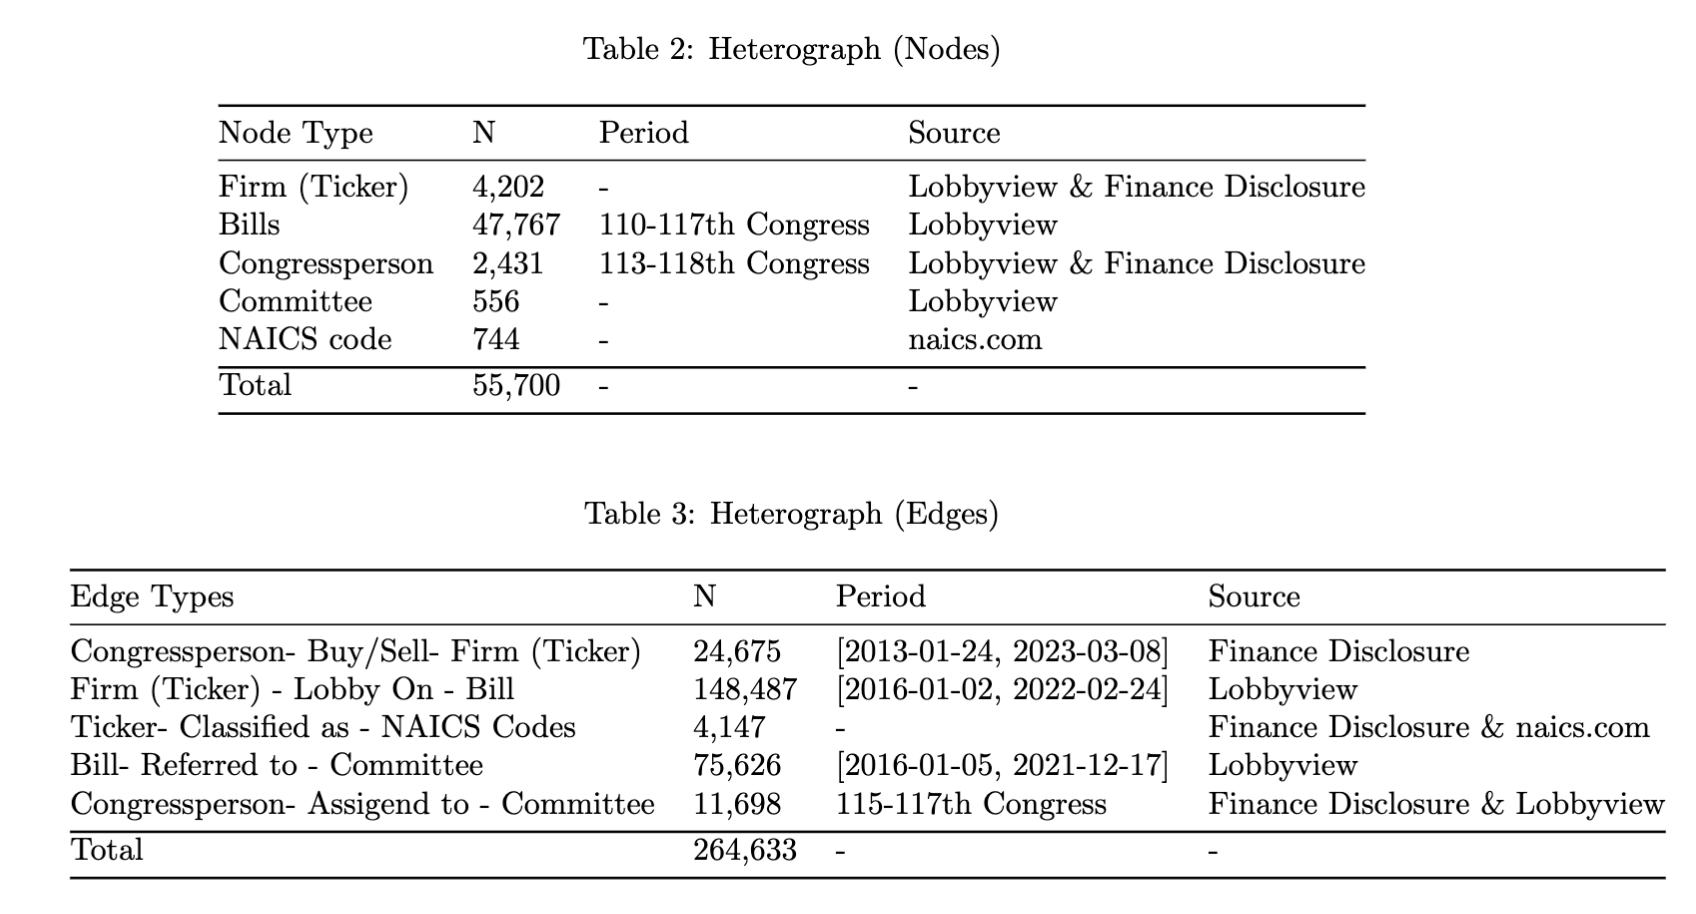
\includegraphics[scale=0.4]{./images/spec.png}

	\end{frame}

	\begin{frame}{Entire Graph}
		\centering	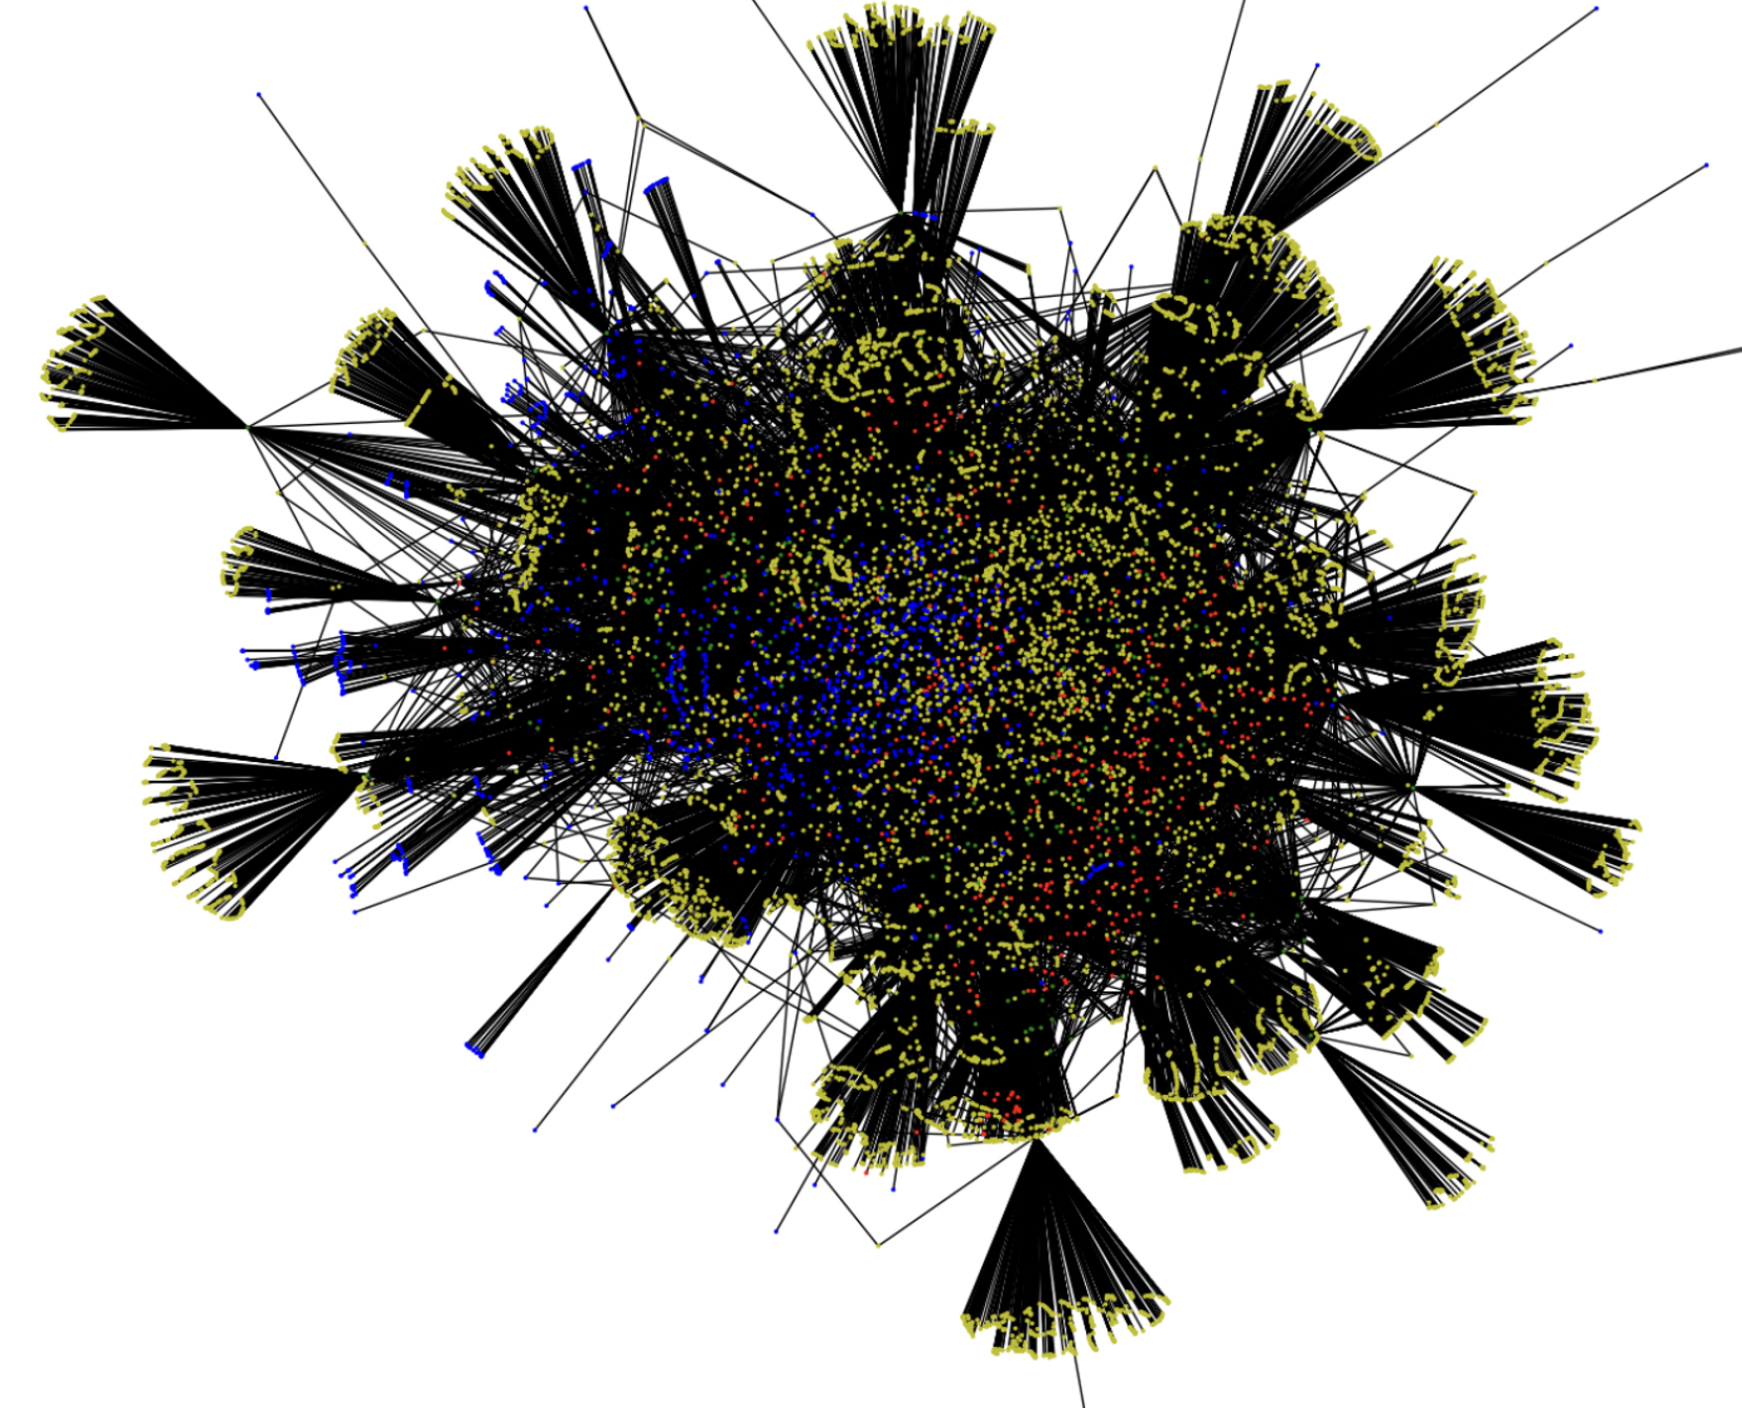
\includegraphics[scale=0.3]{./images/graph.png}
		\\ very dense, hard to interpret
	\end{frame}

	% \begin{frame}{Subgraph Capturing Semiconductor Industry}
	% 	\centering	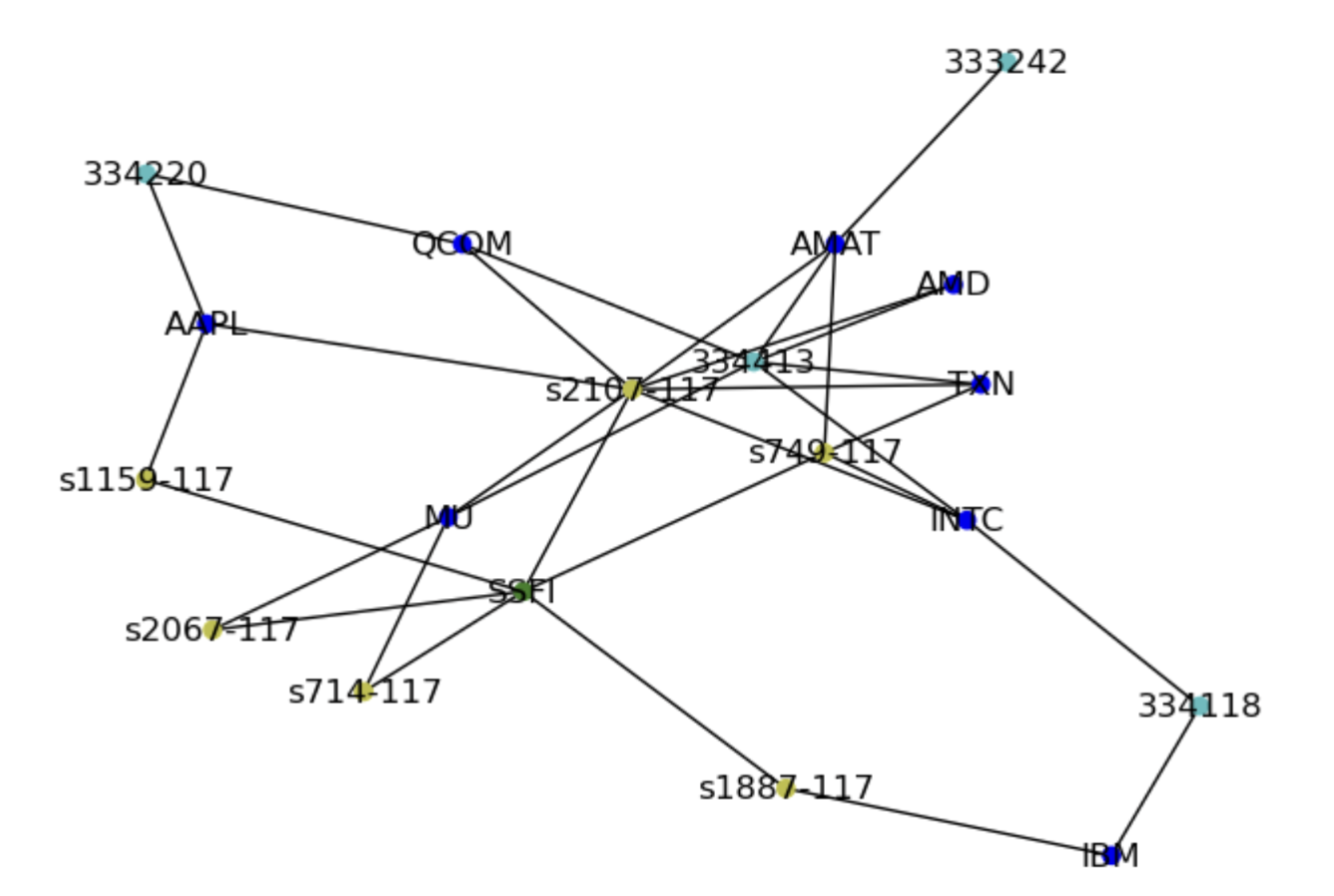
\includegraphics[scale=0.5]{./images/ill.png}
	% \end{frame}

	% \begin{frame}{Subgraph Capturing US Banking Industry}
	% 	\centering	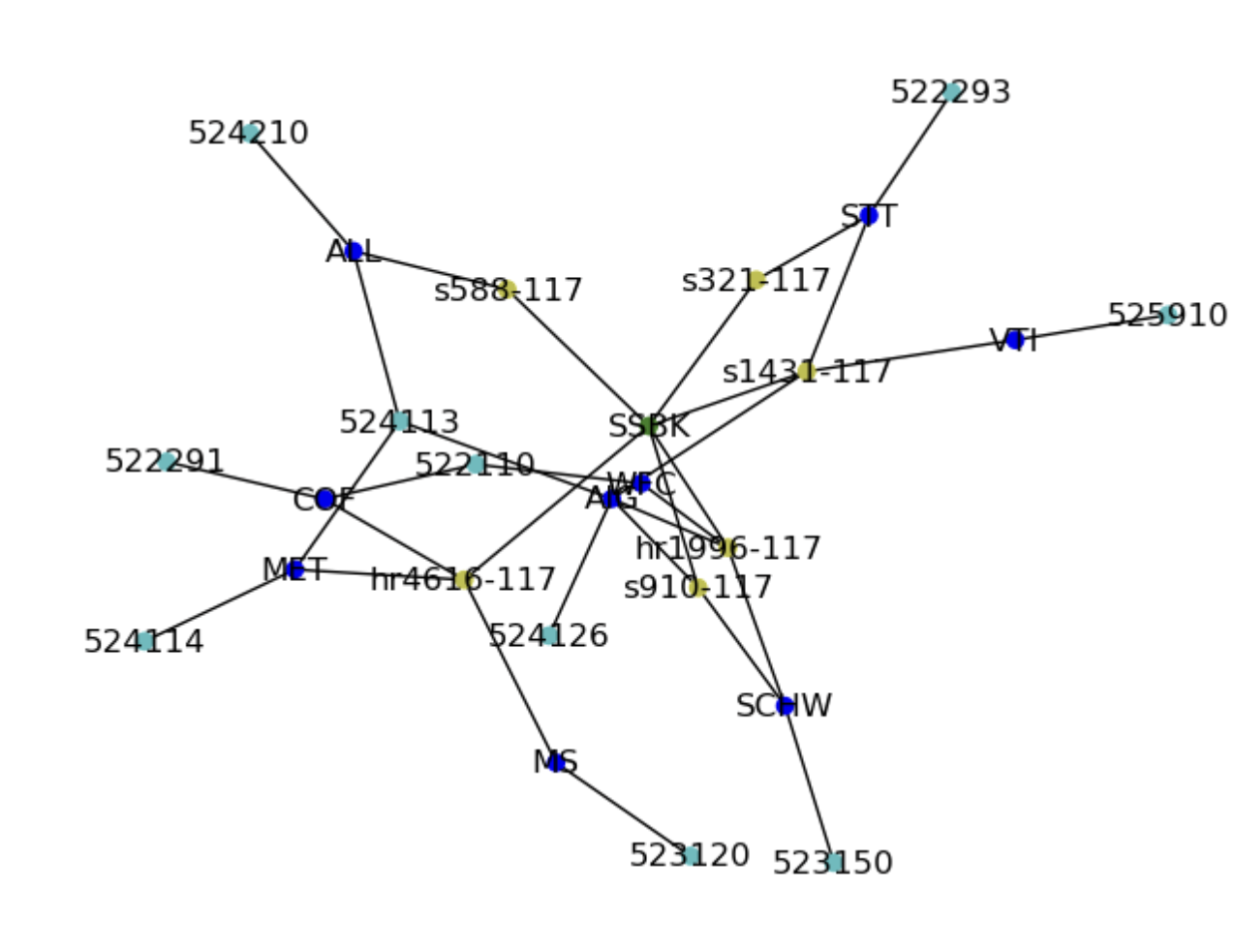
\includegraphics[scale=0.5]{./images/ill2.png}
	% \end{frame}

	\begin{frame}{Industry-Level Specialization}
		\begin{itemize}
			\item Committee specialization can be quantified by aggregating the NAICS codes of firms lobbying on bills referred to the committee.
			\item NAICS PMF of Senate Finance Committee
		\end{itemize}
		\centering	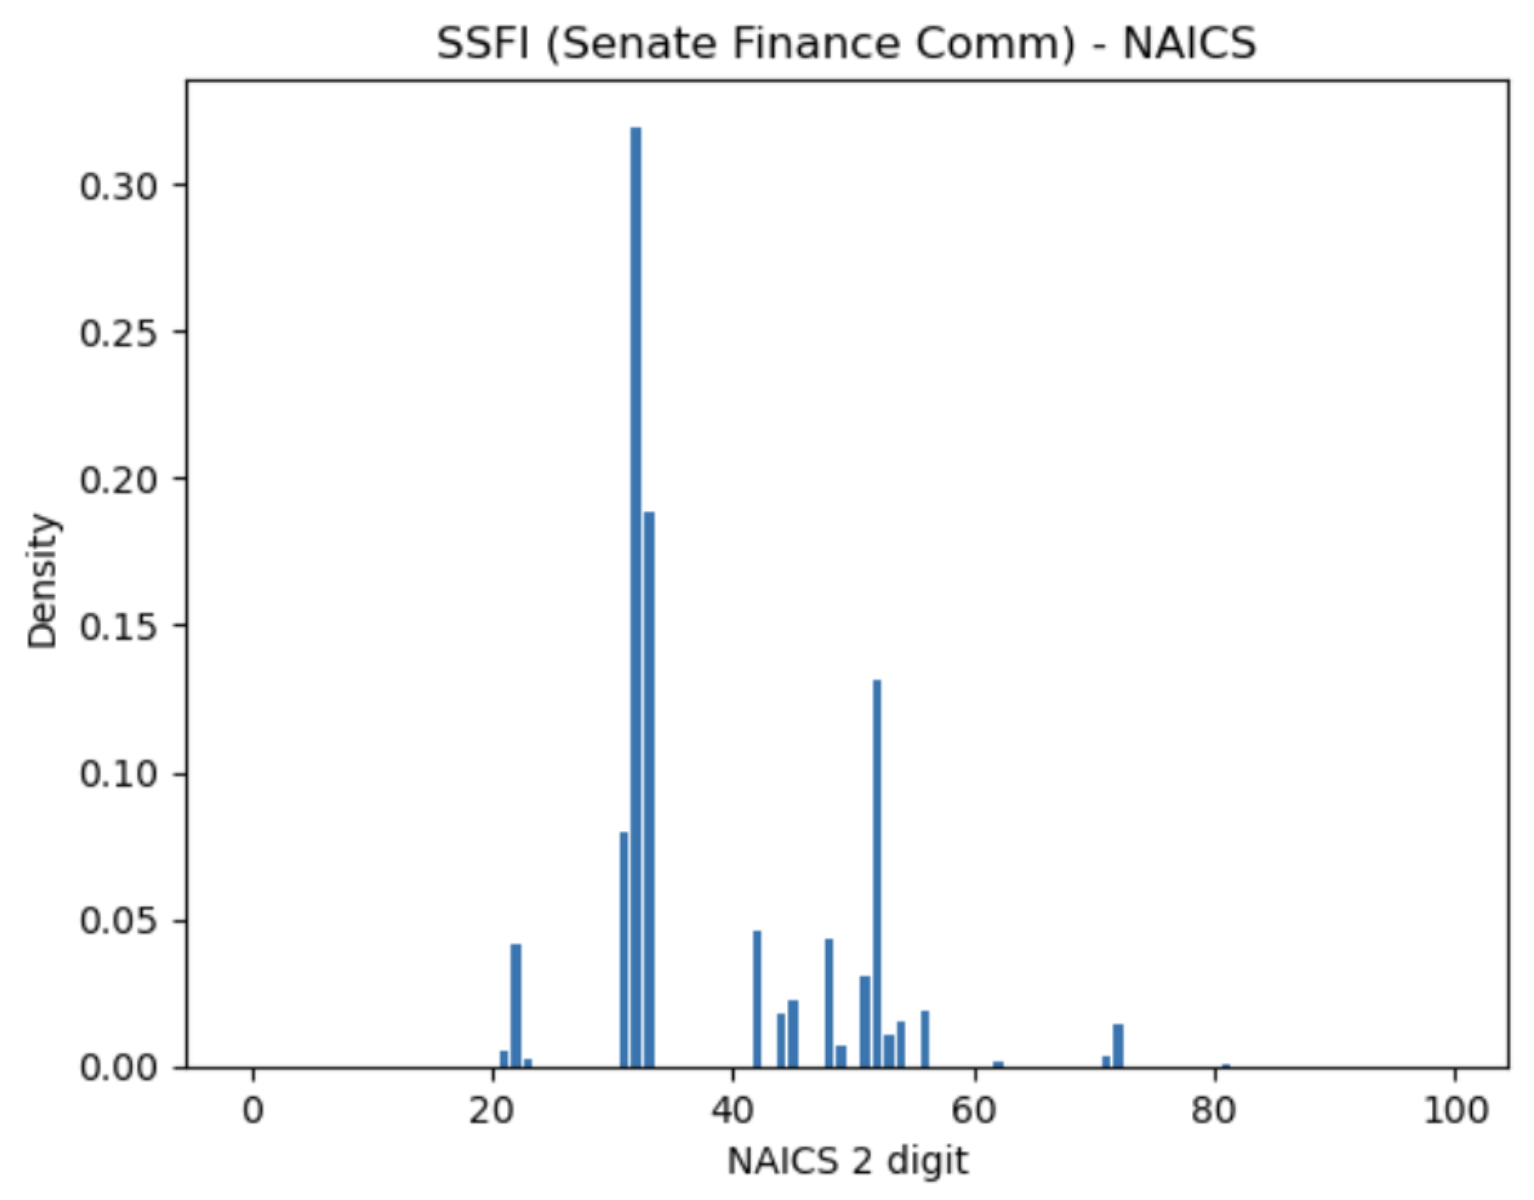
\includegraphics[scale=0.3]{./images/ssfi.png}
	\end{frame}

	\begin{frame}{Industry-Level Specialization}
		\begin{itemize}
			\item NAICS PMF of Senate Banking Committee
		\end{itemize}
		\centering	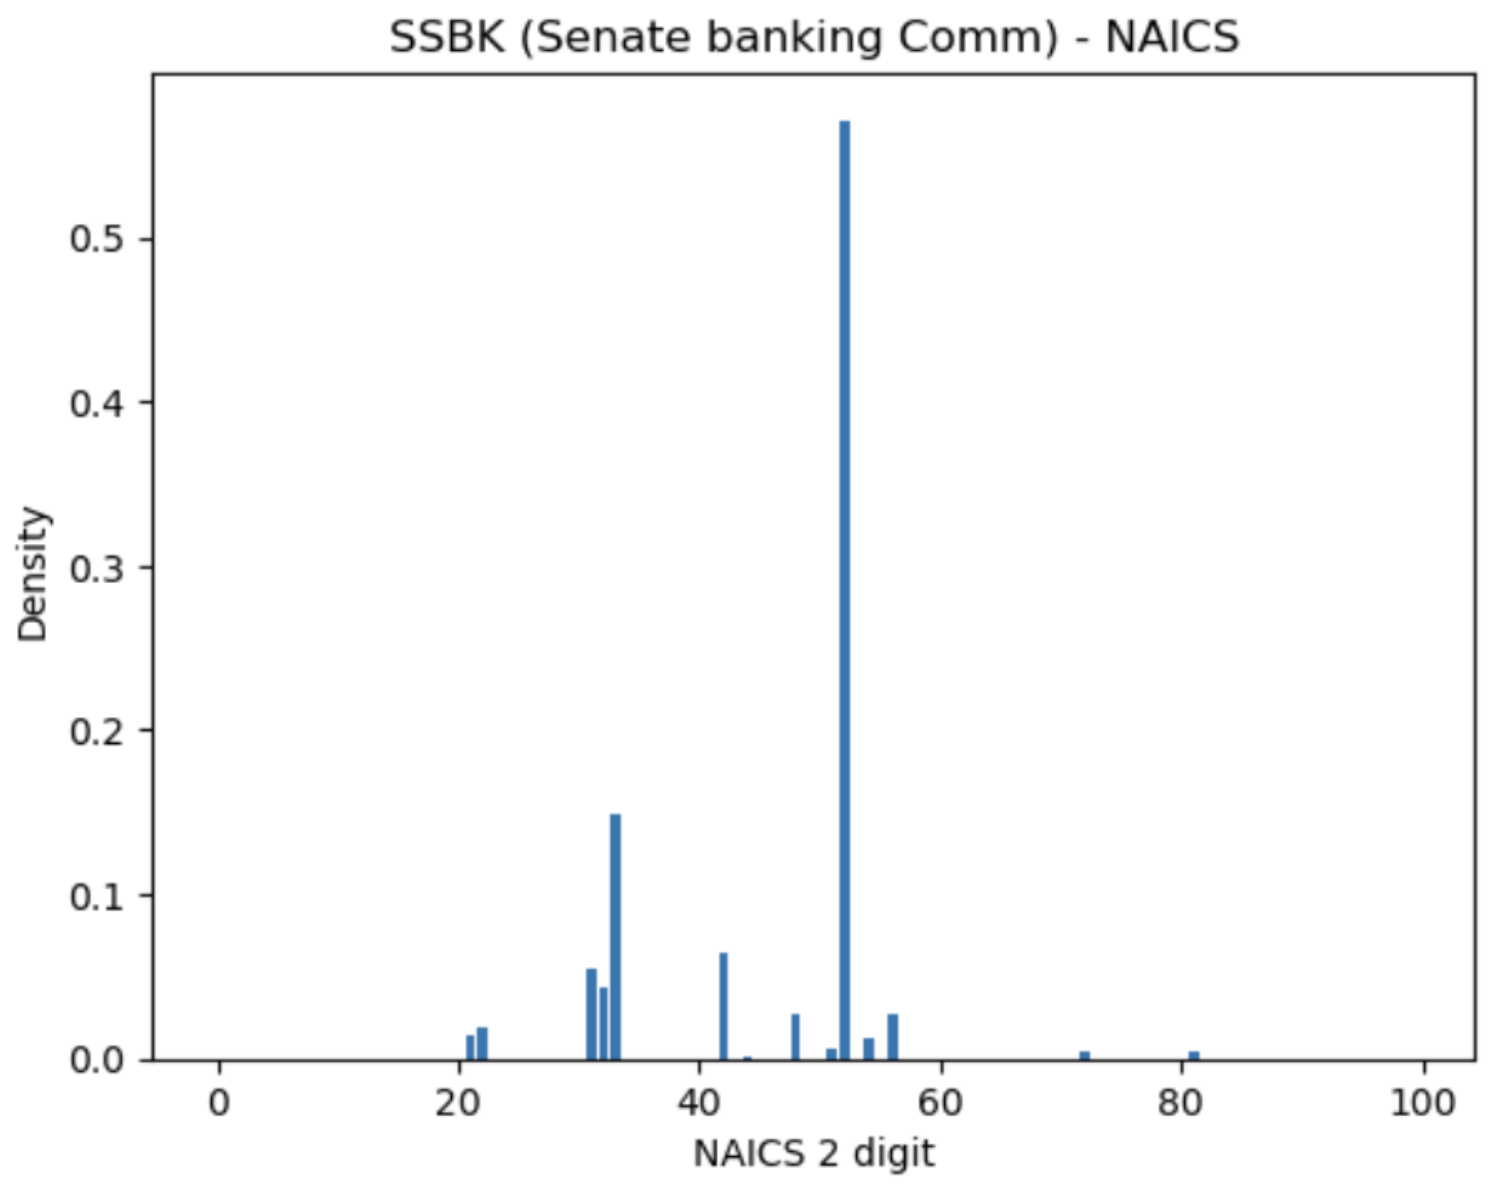
\includegraphics[scale=0.3]{./images/ssbk.png}
	\end{frame}

	\begin{frame}{Industry-Level Specialization}
		\begin{itemize}
			\item Similarly, one can quantify a congressperson's industry-level specialization in their stock portfolio by aggregating the NAICS codes of firms they transacted with.
			\item NAICS PMF of Senator Ron Wyden
		\end{itemize}
		\centering	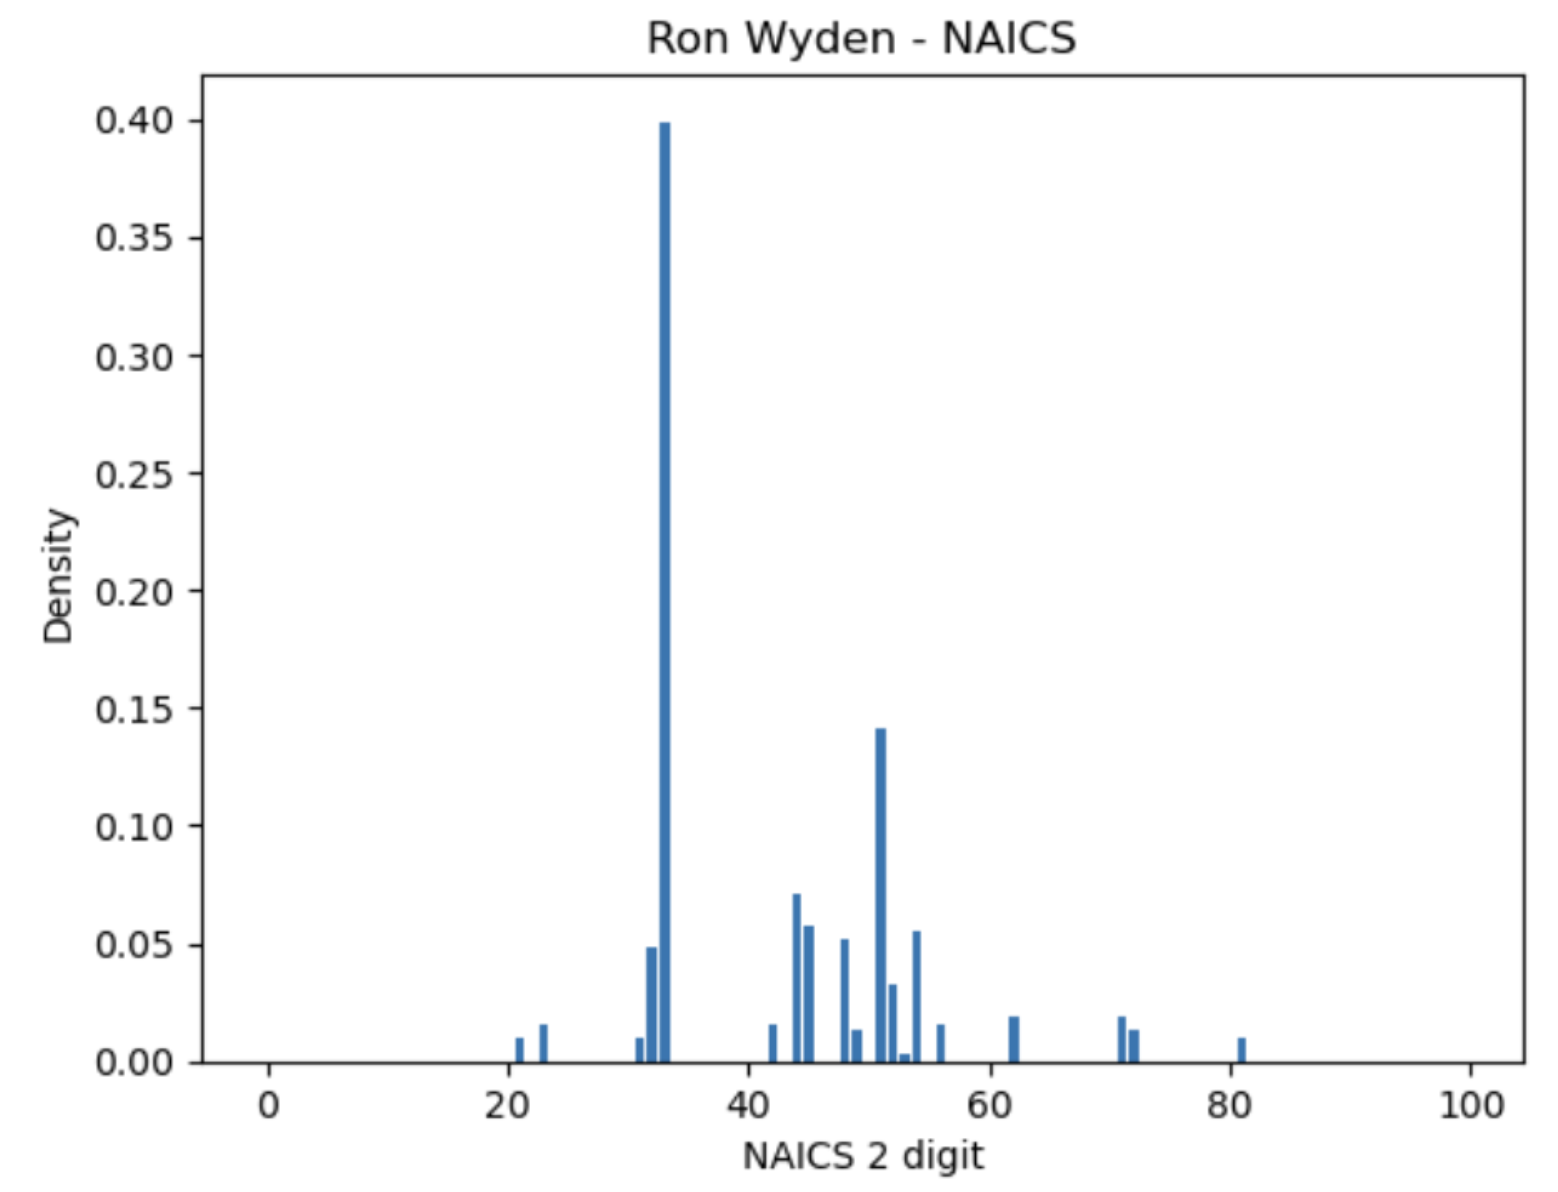
\includegraphics[scale=0.3]{./images/r.png}
	\end{frame}

	\begin{frame}{Industry-Level Specialization}
		\begin{itemize}
			\item We can directly measure the similarity between NAICS PMF of congressperson and committee.
			\item Using Cross-Entropy: $H(P, Q)=-\sum_{x \in \mathcal{X}} p(x) \log q(x)$
			\item Lower, the similar
		\end{itemize}
		\begin{center}
			\begin{minipage}{0.3\textwidth}
				\centering
				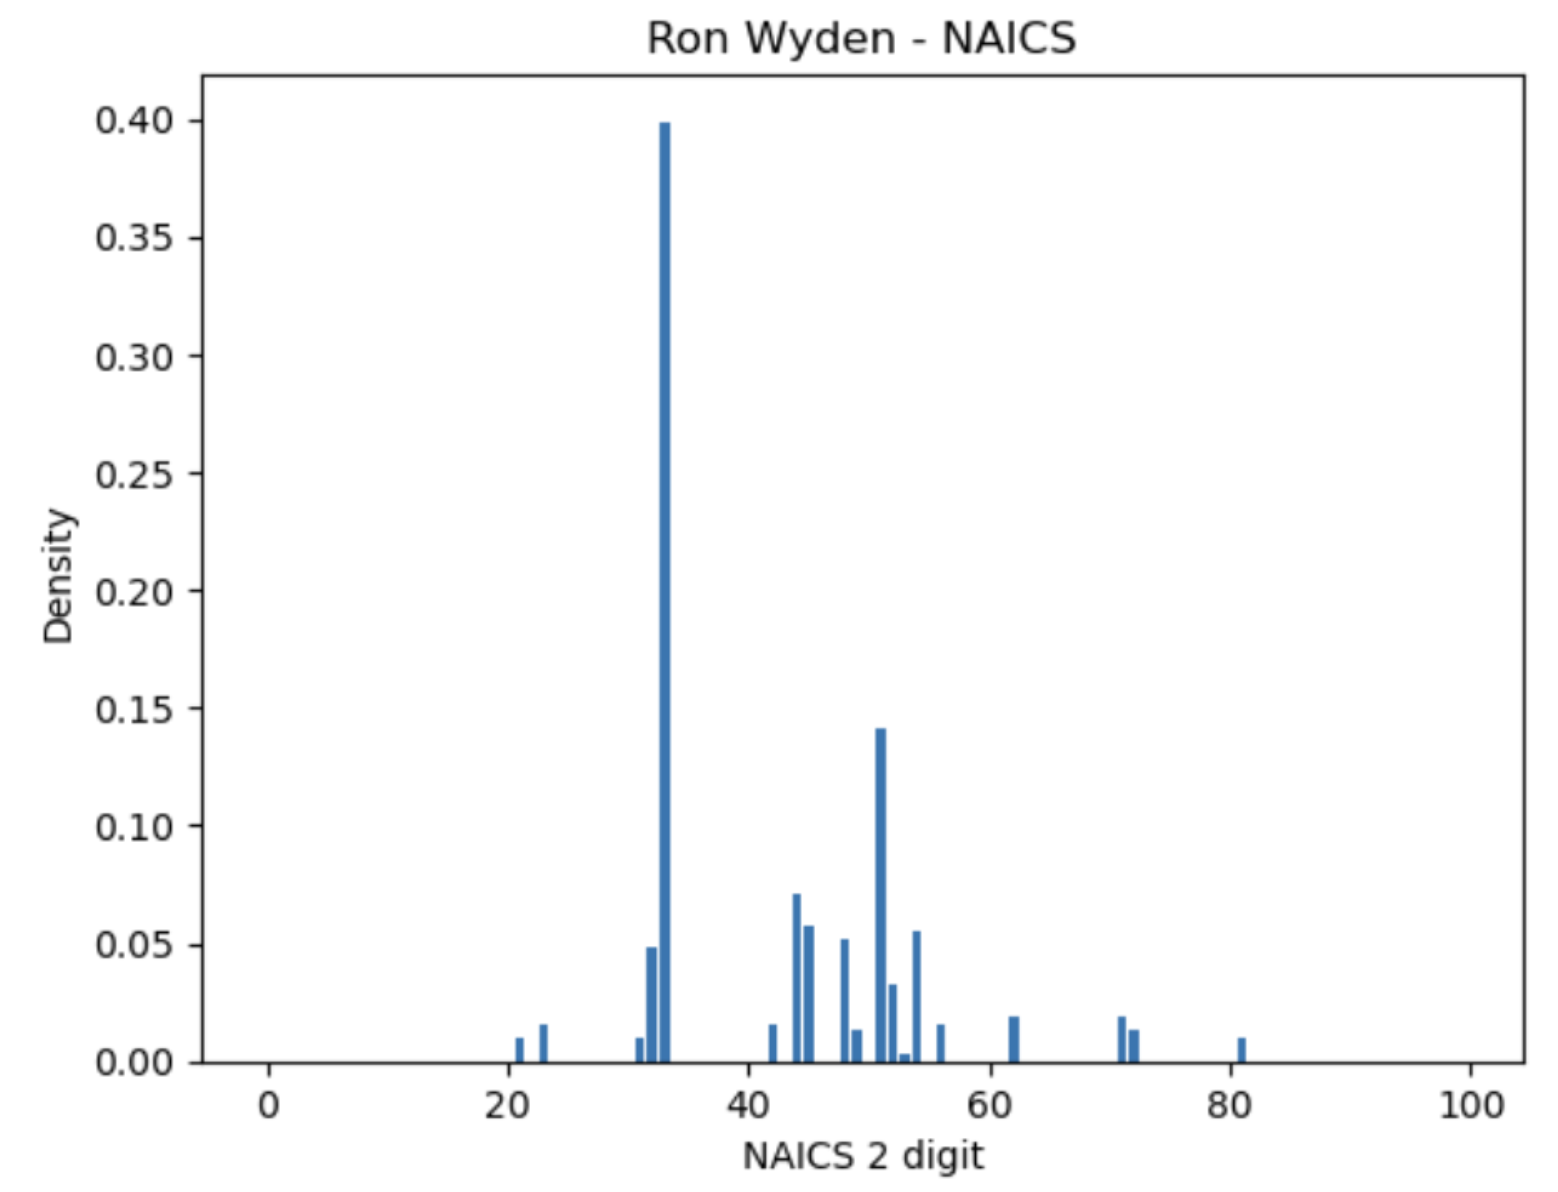
\includegraphics[scale=0.15]{./images/r.png} % First figure
			\end{minipage}
			\hfill
			\begin{minipage}{0.3\textwidth}
				\centering
				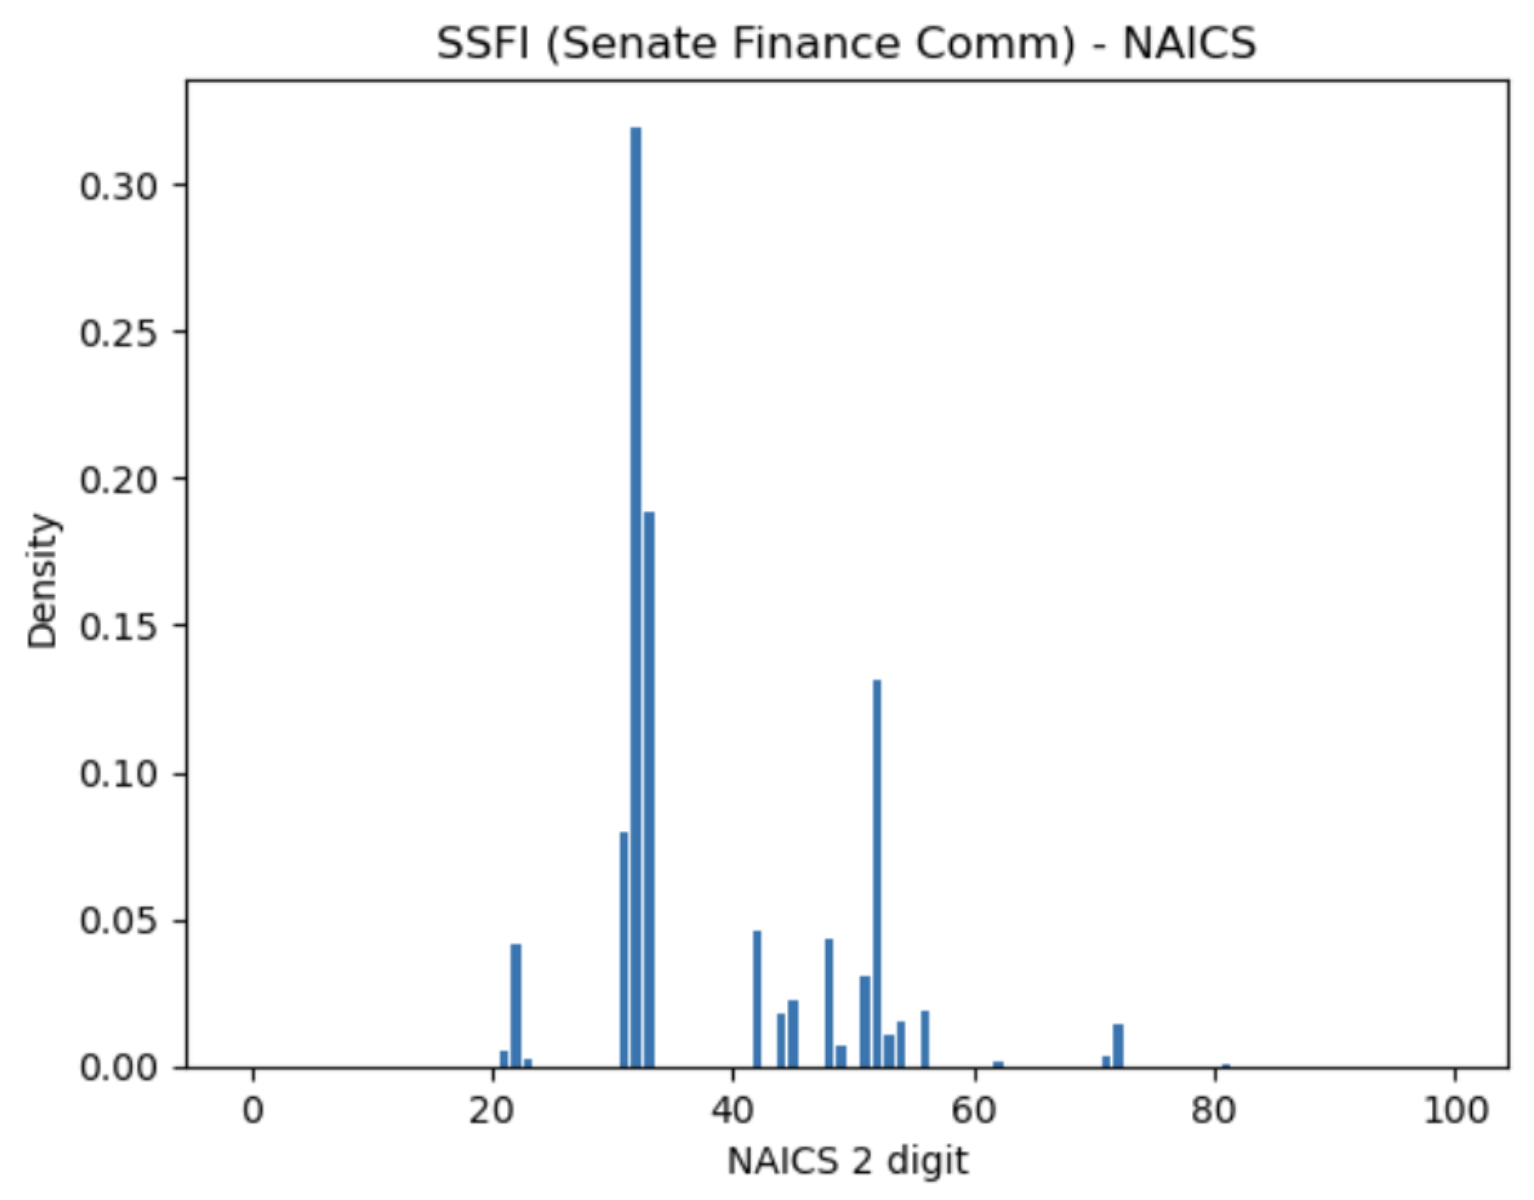
\includegraphics[scale=0.15]{./images/ssfi.png} % Second figure
			\end{minipage}
			\hfill
			\begin{minipage}{0.3\textwidth}
				\centering
				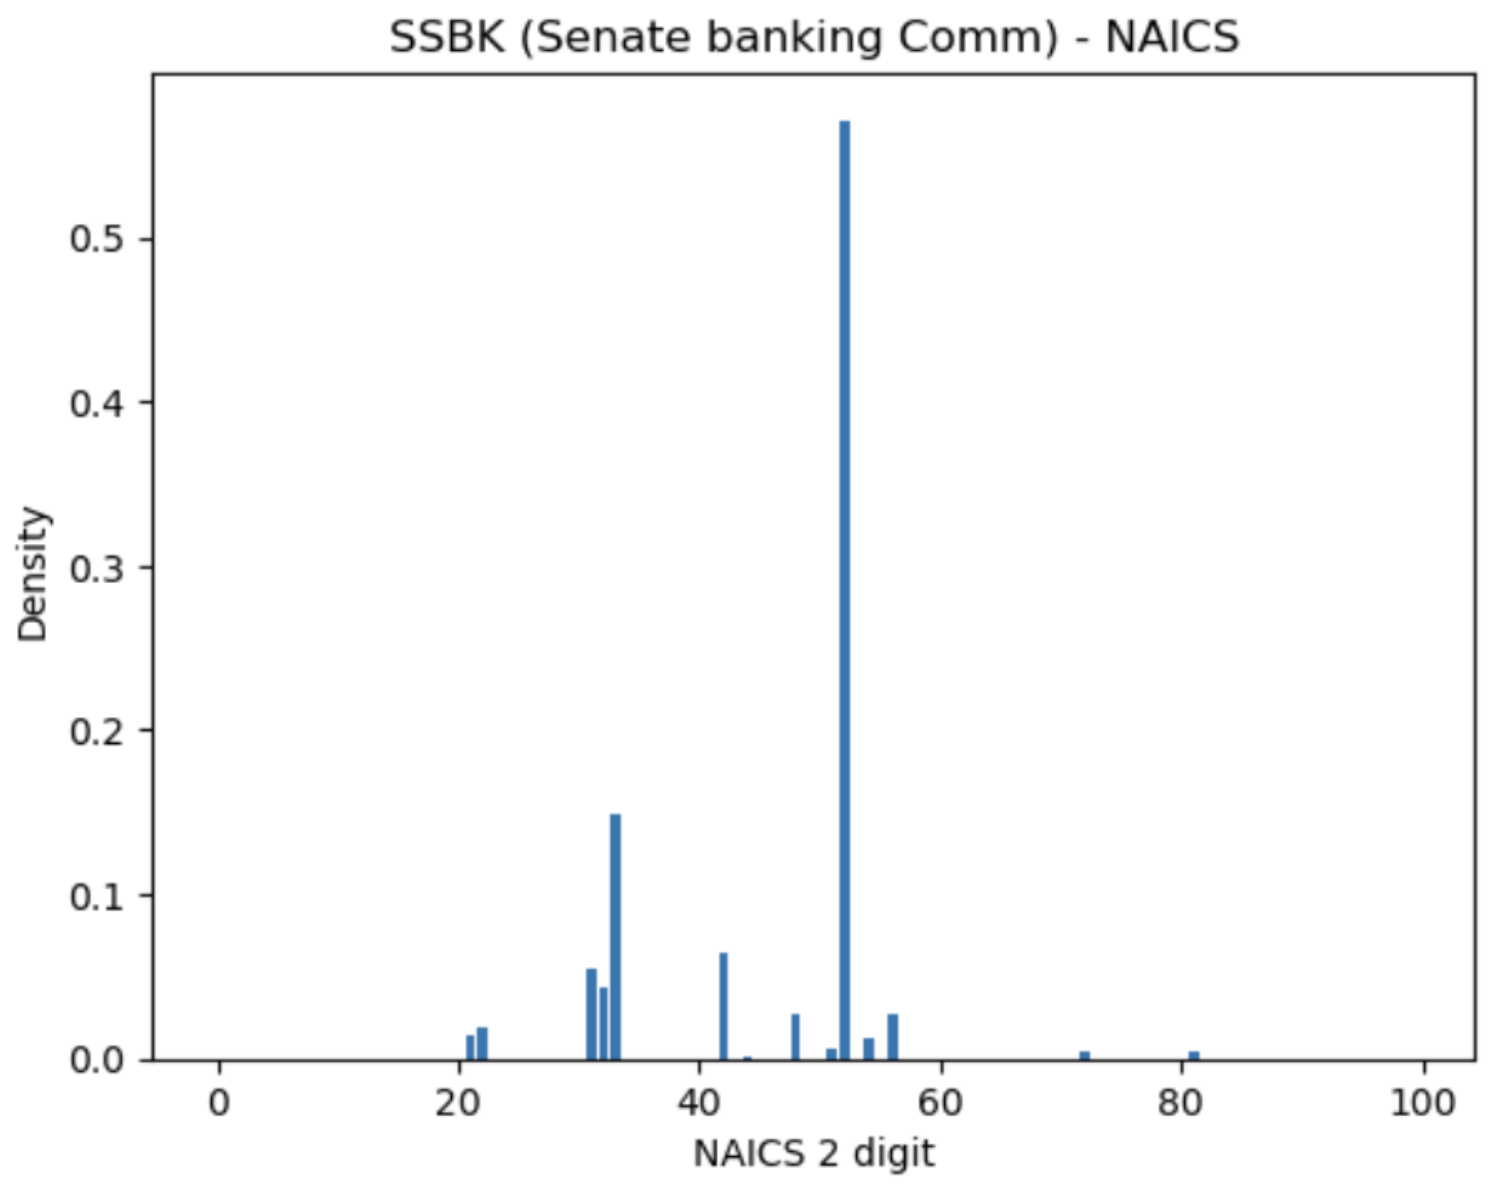
\includegraphics[scale=0.15]{./images/ssbk.png} % Third figure
			\end{minipage}
		\end{center}
		\begin{itemize}
			\item CE(Ron Wyden, SSFI) = 0.7 $<$ CE(Ron Wyden, SSBK) = 3.3
			\item Sen. Ron Wyden is a member of the Senate Committee on Finance
			\item His portfolio resembles the committee's industry specialization
		\end{itemize}
	\end{frame}

	\begin{frame}{Average Cross Entropy: Assinged vs Un-Assigned}
		\centering	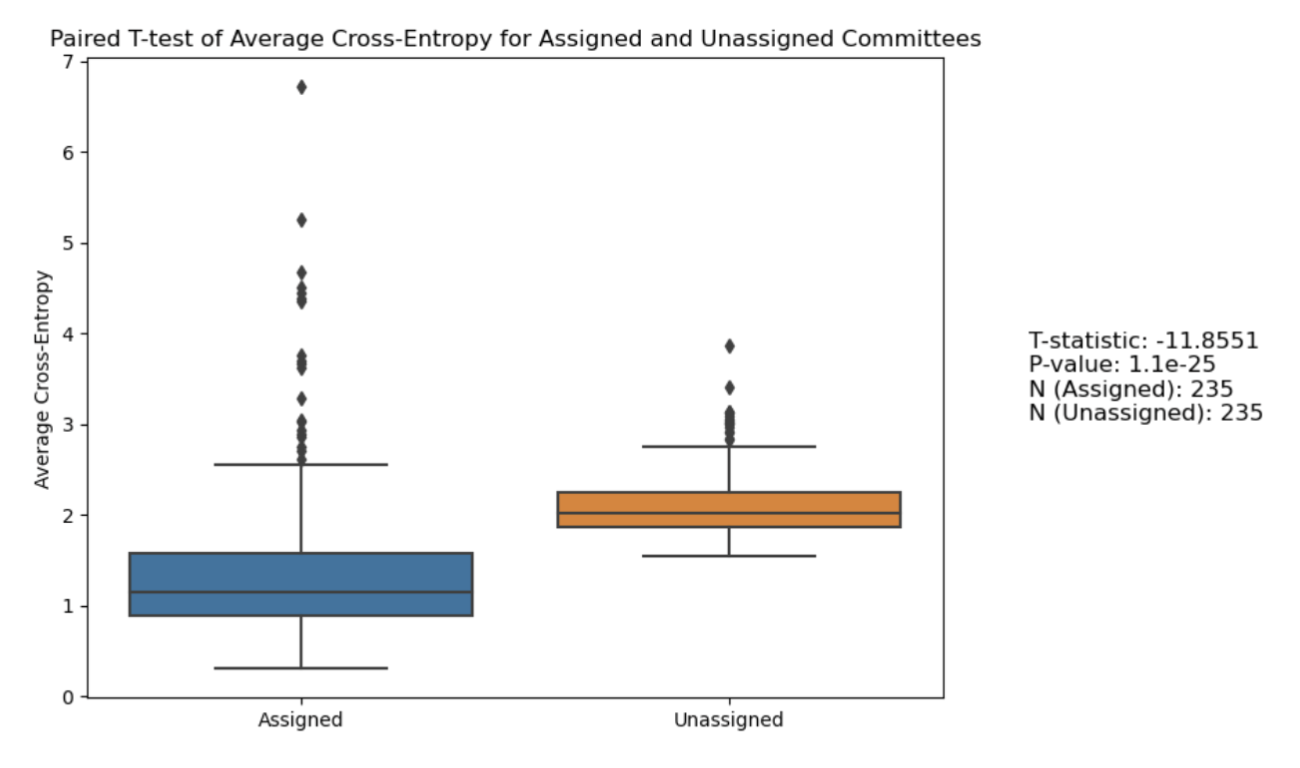
\includegraphics[scale=0.4]{./images/aua.png}
		\begin{itemize}
			\item Congresspeople's stock portfolio resembles their committee's industry specialization
			\item Contrast to Eggers \& Hainmueller (2014) \textit{``we find no evidence that members disproportionately invest in companies to which they are connected through their committee assignments.''}
		\end{itemize}
	\end{frame}

	\begin{frame}{Predictive Modeling: Graph $\rightarrow$ Transaction}

		Egger \& Hainmueller (2014) model:
		$$w_{i j}=\alpha+\beta_1 \text { District }_{i j}+\beta_2 \text { Contributions }_{i j}+\beta_3 \text { Lobbying }_{i j}+\theta_i+\theta_j+\varepsilon_{i j}$$

		\begin{itemize}
			\item $w_{ij}$ is portfolio weight of a firm $j$ for congressperson $i$
			\item How predictive is the graph for stock transactions? 
		\end{itemize}

	\end{frame}	

	\begin{frame}{Link Prediction using Graph Neural Network}
		\begin{itemize}
			\item Link prediction is a task of predicting the existence of a link between two nodes in a graph
			\item Given two nodes $u$ and $v$, we want to predict whether there is an edge between them
			\item $u$ is a congressperson and $v$ is a firm (ticker)
		\end{itemize}
\centering	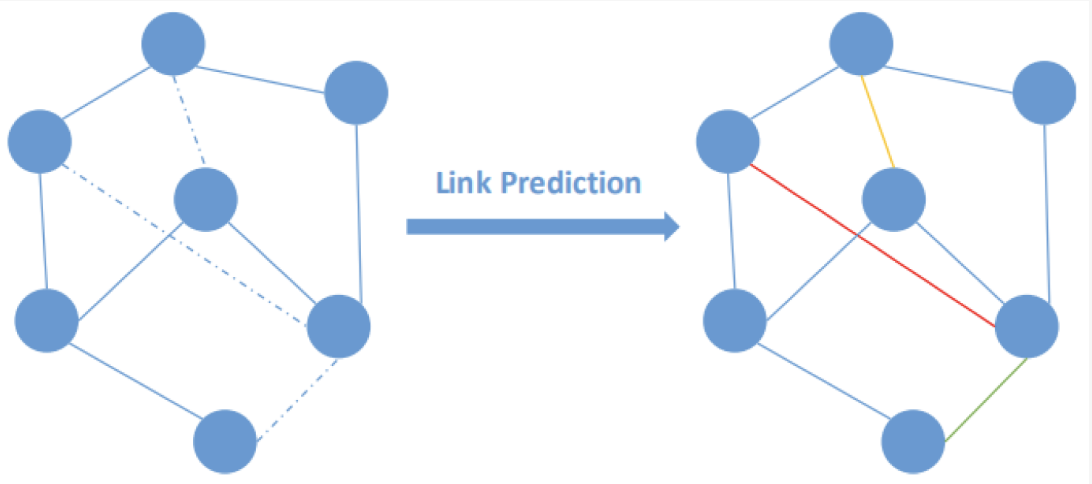
\includegraphics[scale=0.4]{./images/linkpred.png}
	\end{frame}	

	\begin{frame}{Link Prediction using Graph Neural Network}
		Idea is similar to logistic regression:
		$$
\pi_i=\operatorname{sigmoid}\left(X_i^{\top} \beta\right) \equiv \frac{\exp \left(X_i^{\top} \beta\right)}{1+\exp \left(X_i^{\top} \beta\right)}
$$
where $\pi_i \in [0, 1]$
		\begin{itemize}
			\item Replace $X_i^{\top} \beta$ (logit) with $PredHead(h_{congressperson}, h_{ticker})$
			\item $PredHead$ is normally a dot product or a neural network
			\item $h_{congressperson}, h_{ticker}$ are multi-dimensional vectors that represents each node (similar idea like D(W)-Nominate score)
			\item How to learn $h_{congressperson}, h_{ticker}$ to encode the information embedded in the graph structured data? 
			\item Using Graph Neural Network (GNN)
			\item GNN should map $h_{congressperson}, h_{ticker}$ into a close distance if they are connected in the graph
		\end{itemize}

	\end{frame}	


	\begin{frame}{GNN Architecture}
		I used Edge-Conditioned Convolution (Simonovsky, 2017)
		$$
\mathbf{h}_i^{\prime}=\mathbf{\Theta} \mathbf{h}_i+\sum_{j \in \mathcal{N}(i)} \mathbf{M L P}\left(\mathbf{e}_{i, j}\right) \cdot \mathbf{h}_j
$$
		\begin{itemize}
			\item GNN is computation graph of iteratively updating node representations
			\item Message Passing, Aggreagation, and Update
		\end{itemize}
		\centering	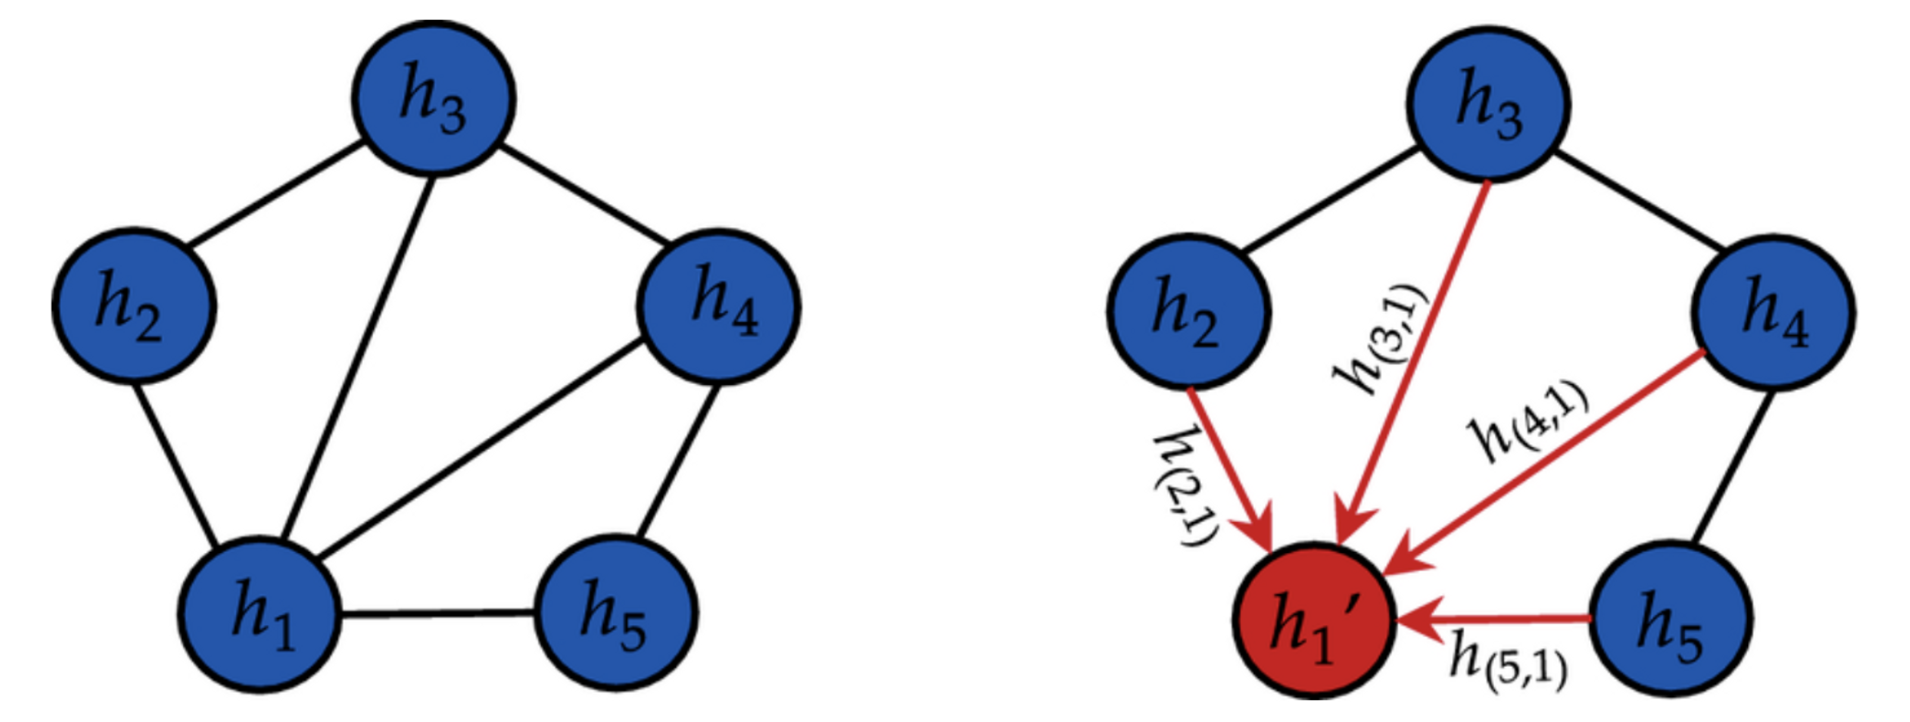
\includegraphics[scale=0.3]{./images/mp.png}
	\end{frame}	

	\begin{frame}{Training and Evaluation}
		\begin{itemize}
			\item Total 24,675 edges for edge-type (congressperson, buy/sell, ticker)
			\item 80\% of the edges are used for training, 20\% for testing
			\item Same number of negative edges are sampled for training (Negative Sampling; For balanced training)
			\item 5-fold cross validation for uncertainty statistics
			\item Ablation study for feature importance - removing each edge-types and see how the performance changes
		\end{itemize}
	\end{frame}

	\begin{frame}{Performance: Accuracy}
		\centering	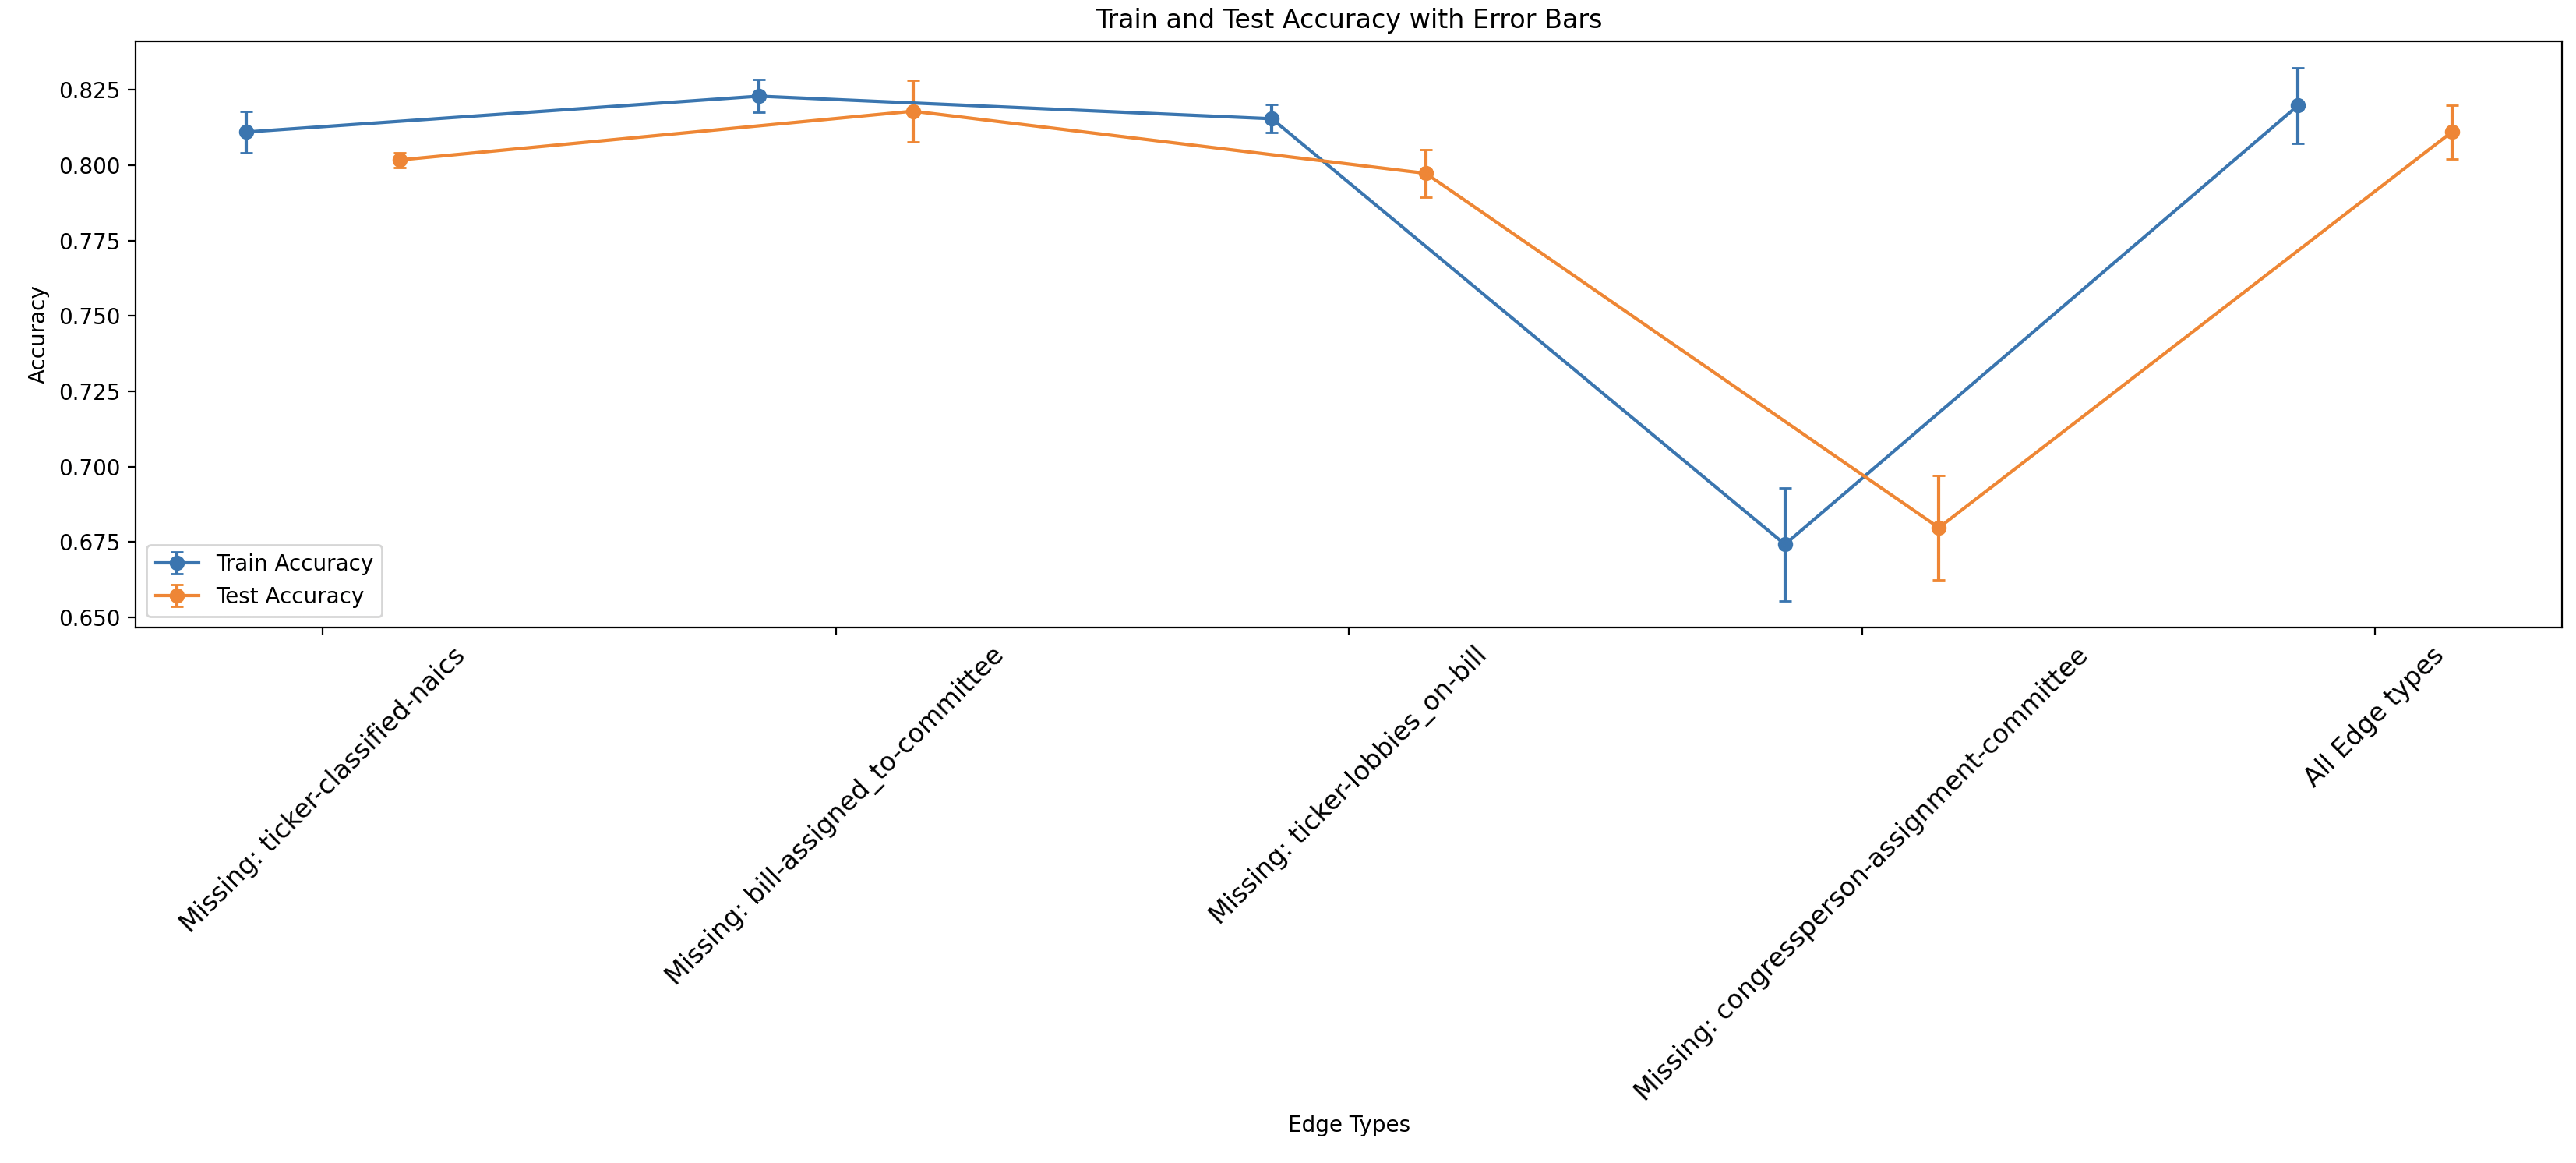
\includegraphics[scale=0.22]{./images/acc2.png}\\
		Use All Edge Types: 82\% accuracy \\
		Remove Committee Assignments of MC: 65\% accuracy
	\end{frame}

	\begin{frame}{Performance: AUC-ROC}
		\centering	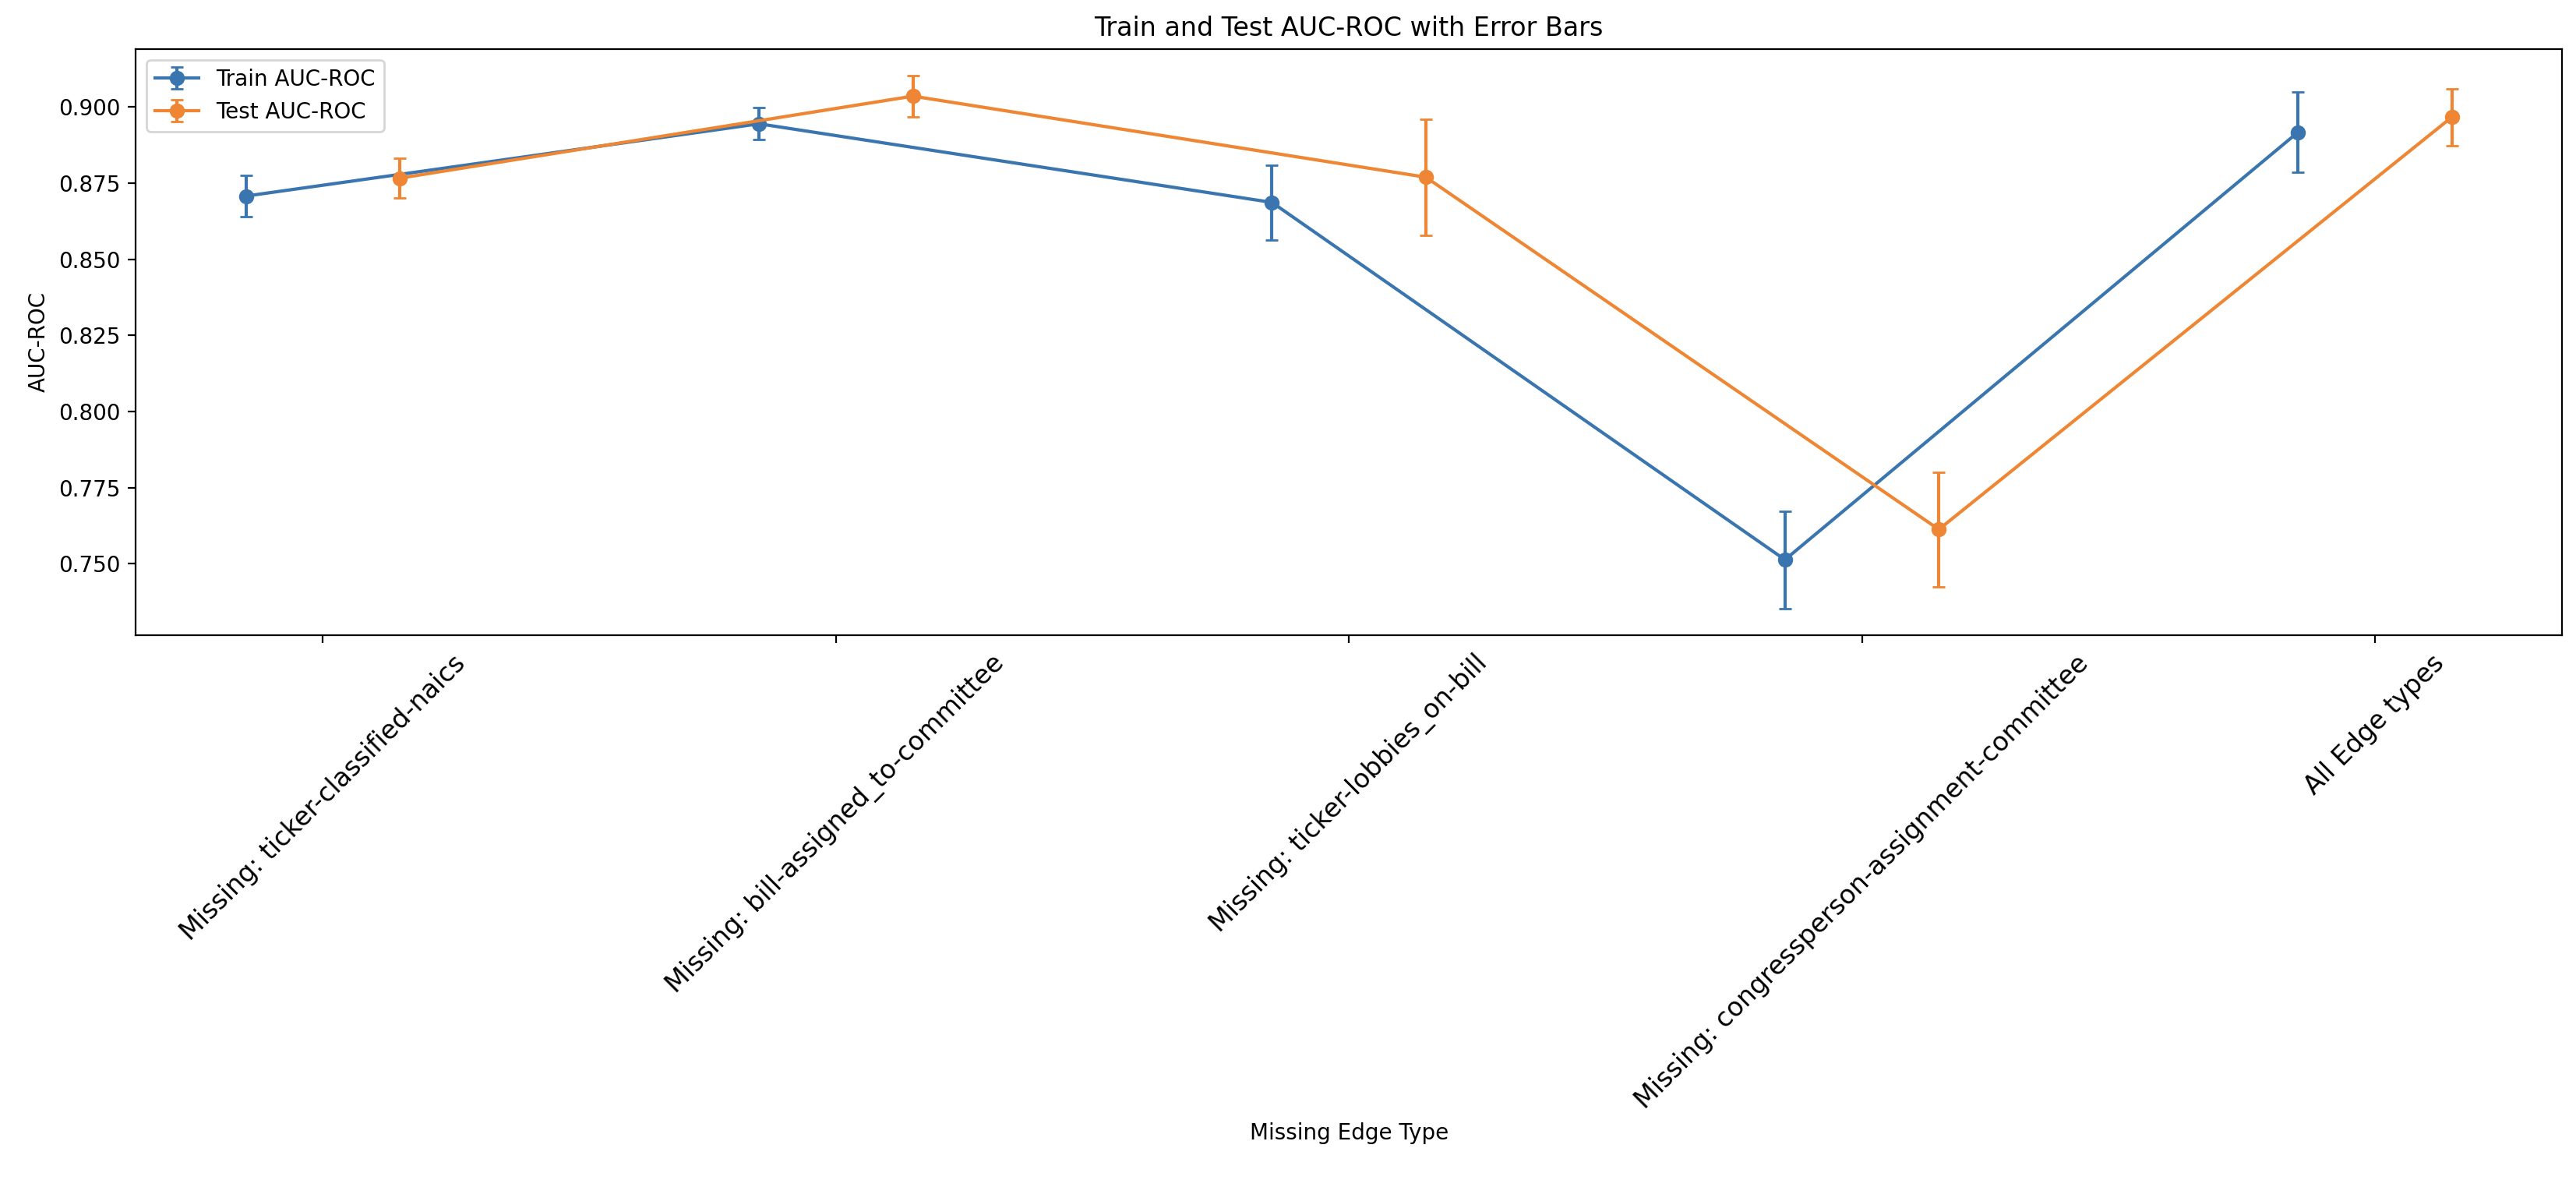
\includegraphics[scale=0.22]{./images/auc2.png}

		\begin{itemize}
			\item The performance drops the most when we remove the committee assignments for congresspersons.
			\item Committee assignments are the most important feature for predicting stock trading by congresspersons. 
		\end{itemize}
	\end{frame}

	\begin{frame}{Shapley Value}
		$$
\varphi_i(v)=\sum_{S \subseteq N \backslash\{i\}} \frac{|S| !(n-|S|-1) !}{n !}(v(S \cup\{i\})-v(S))
$$
		\begin{itemize}
			\item Shapley value represents the fair contribution or importance of each player
			\item Shapley value can be applied to compute the significance of different edge types in link prediction task
			\item Measure: How much each edge type contributes to the prediction?
			\item Can be computed by $16 (=2^4)$ different combinations of $4$ edge types
		\end{itemize}
	\end{frame}

	\begin{frame}{Shapley Value}
		\centering	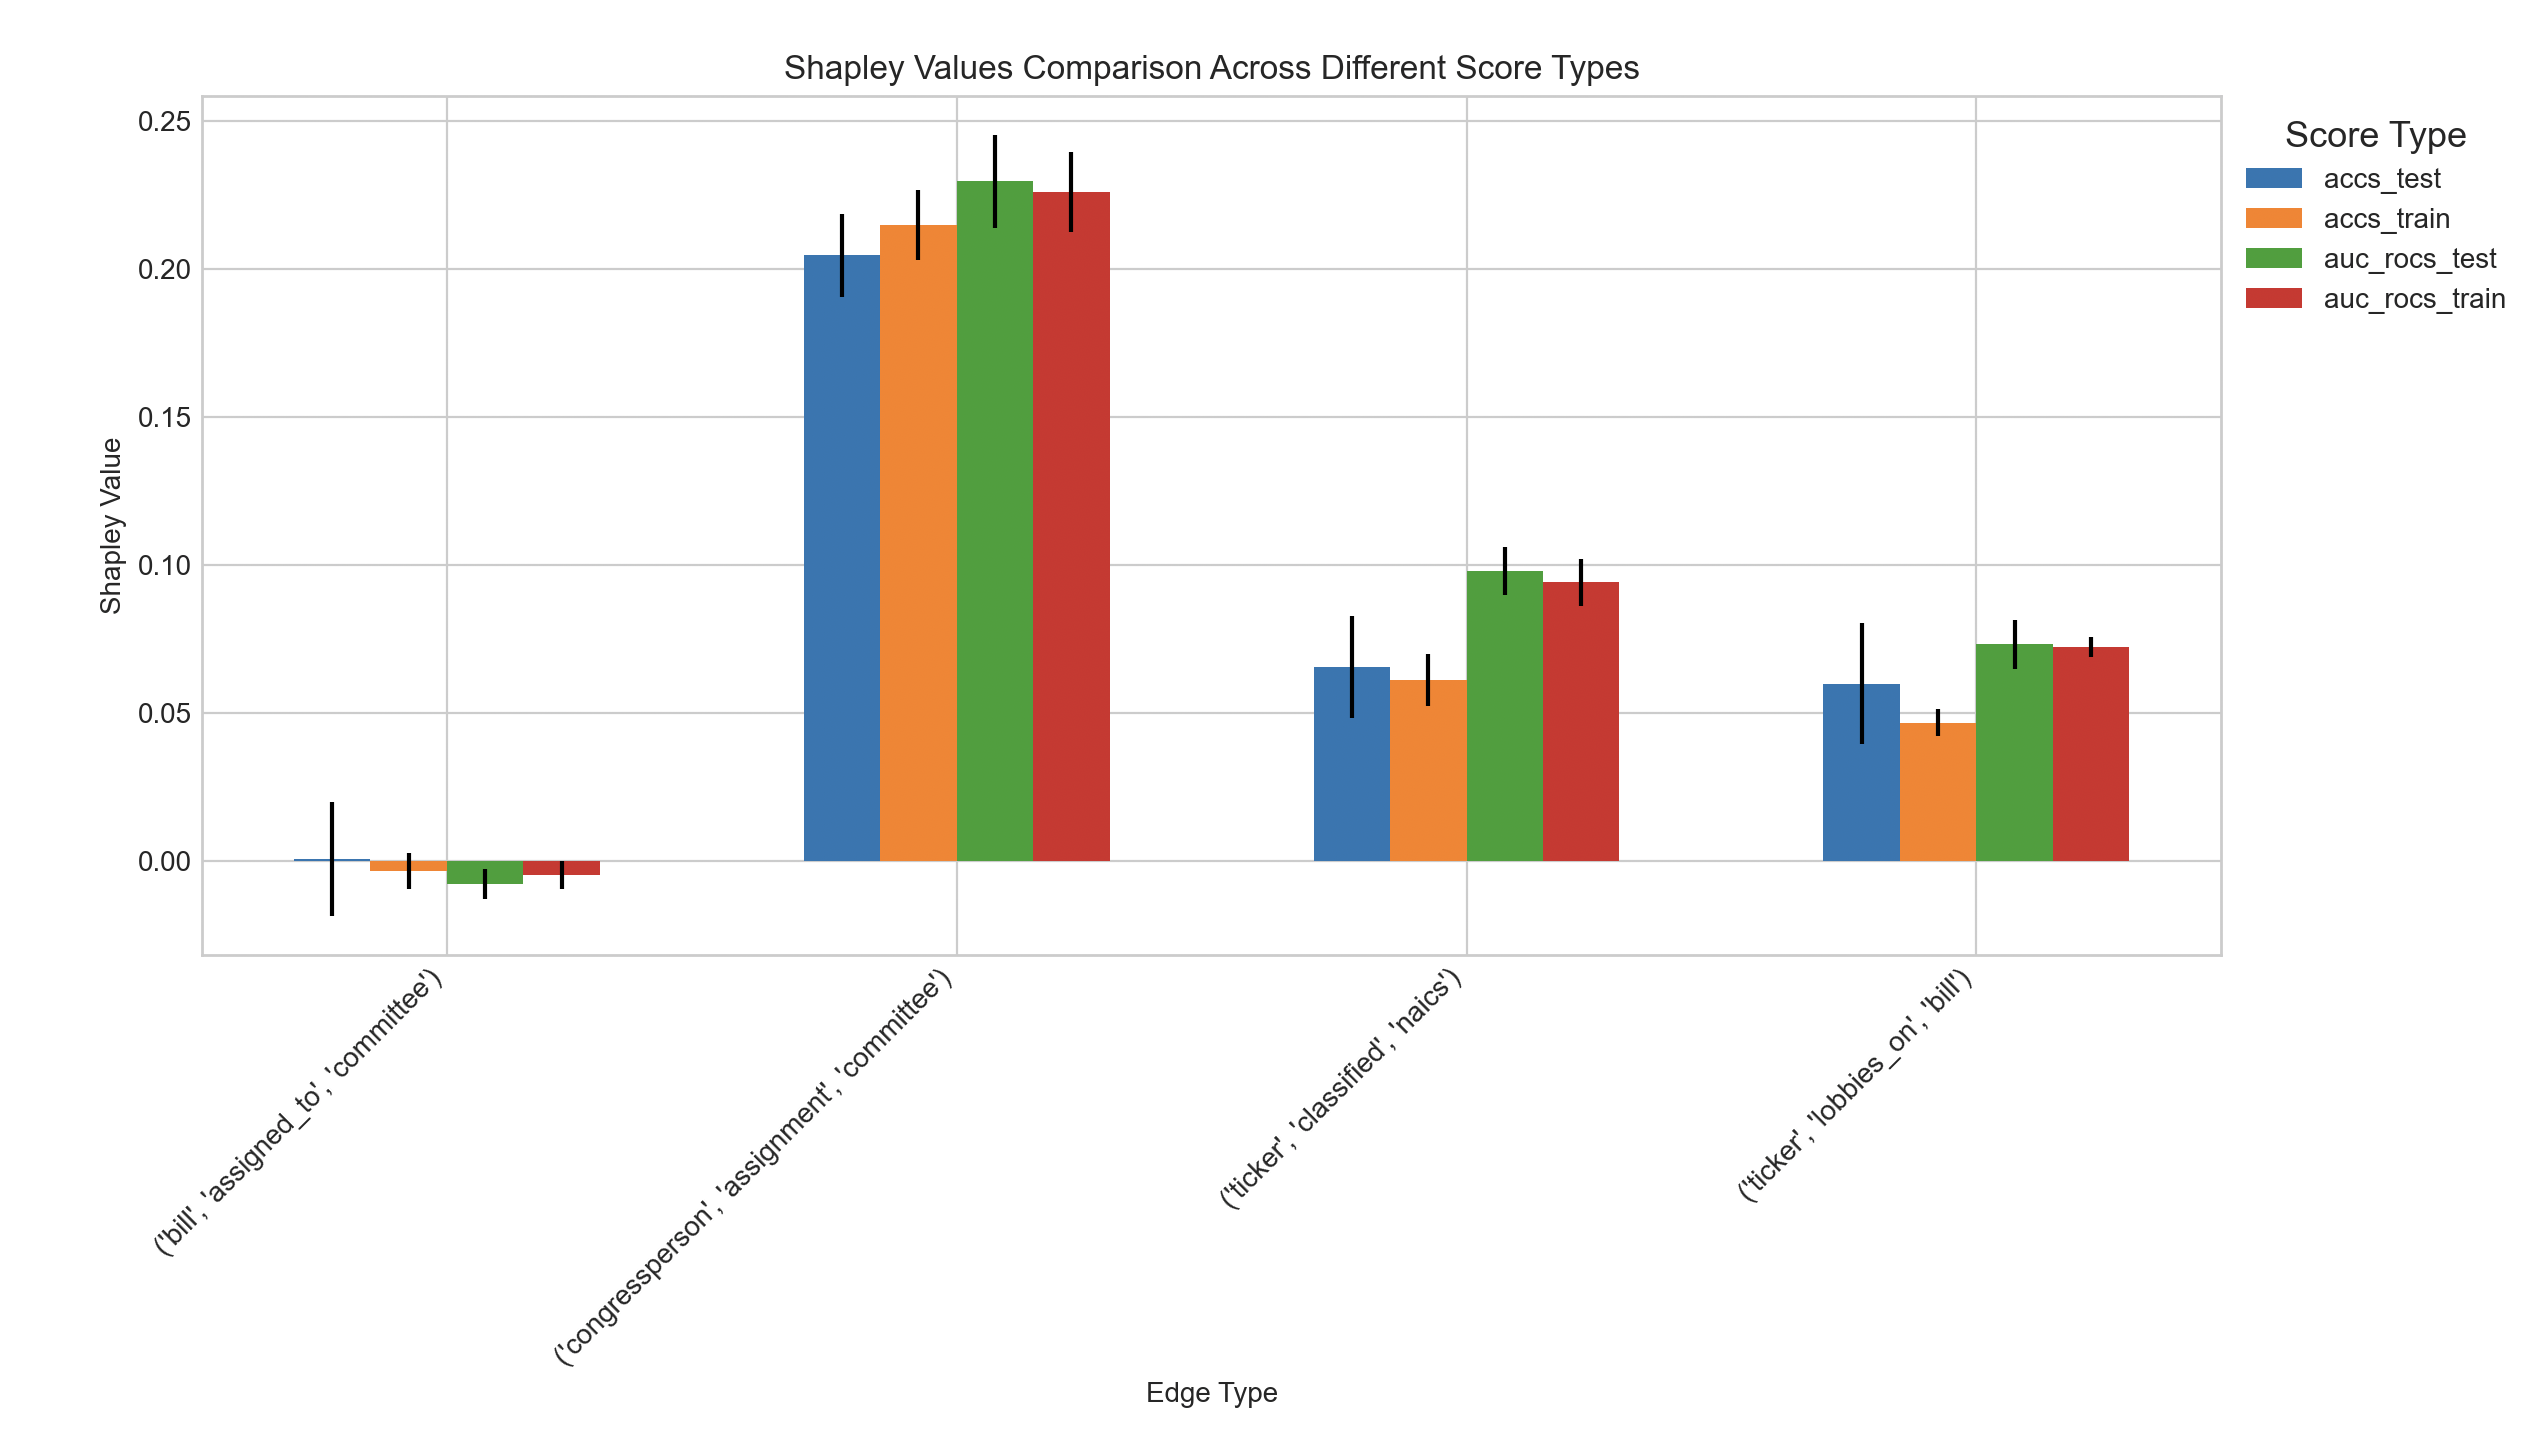
\includegraphics[scale=0.21]{./images/shap.png}

		\begin{itemize}
			\item Committee assignment is key for predicting congresspersons' stock trading.
			\item Firm lobbying on bills and NAICS code also matter.
			\item Bill referral to committees isn't helpful—it hurts performance.
			\item Incomplete Lobbyview data could be a factor - Parsing bills from lobbying reports is hard.
		\end{itemize}
	\end{frame}

	\begin{frame}{GNNExplainer}
		Which nodes and edges are important for the prediction?
		\centering	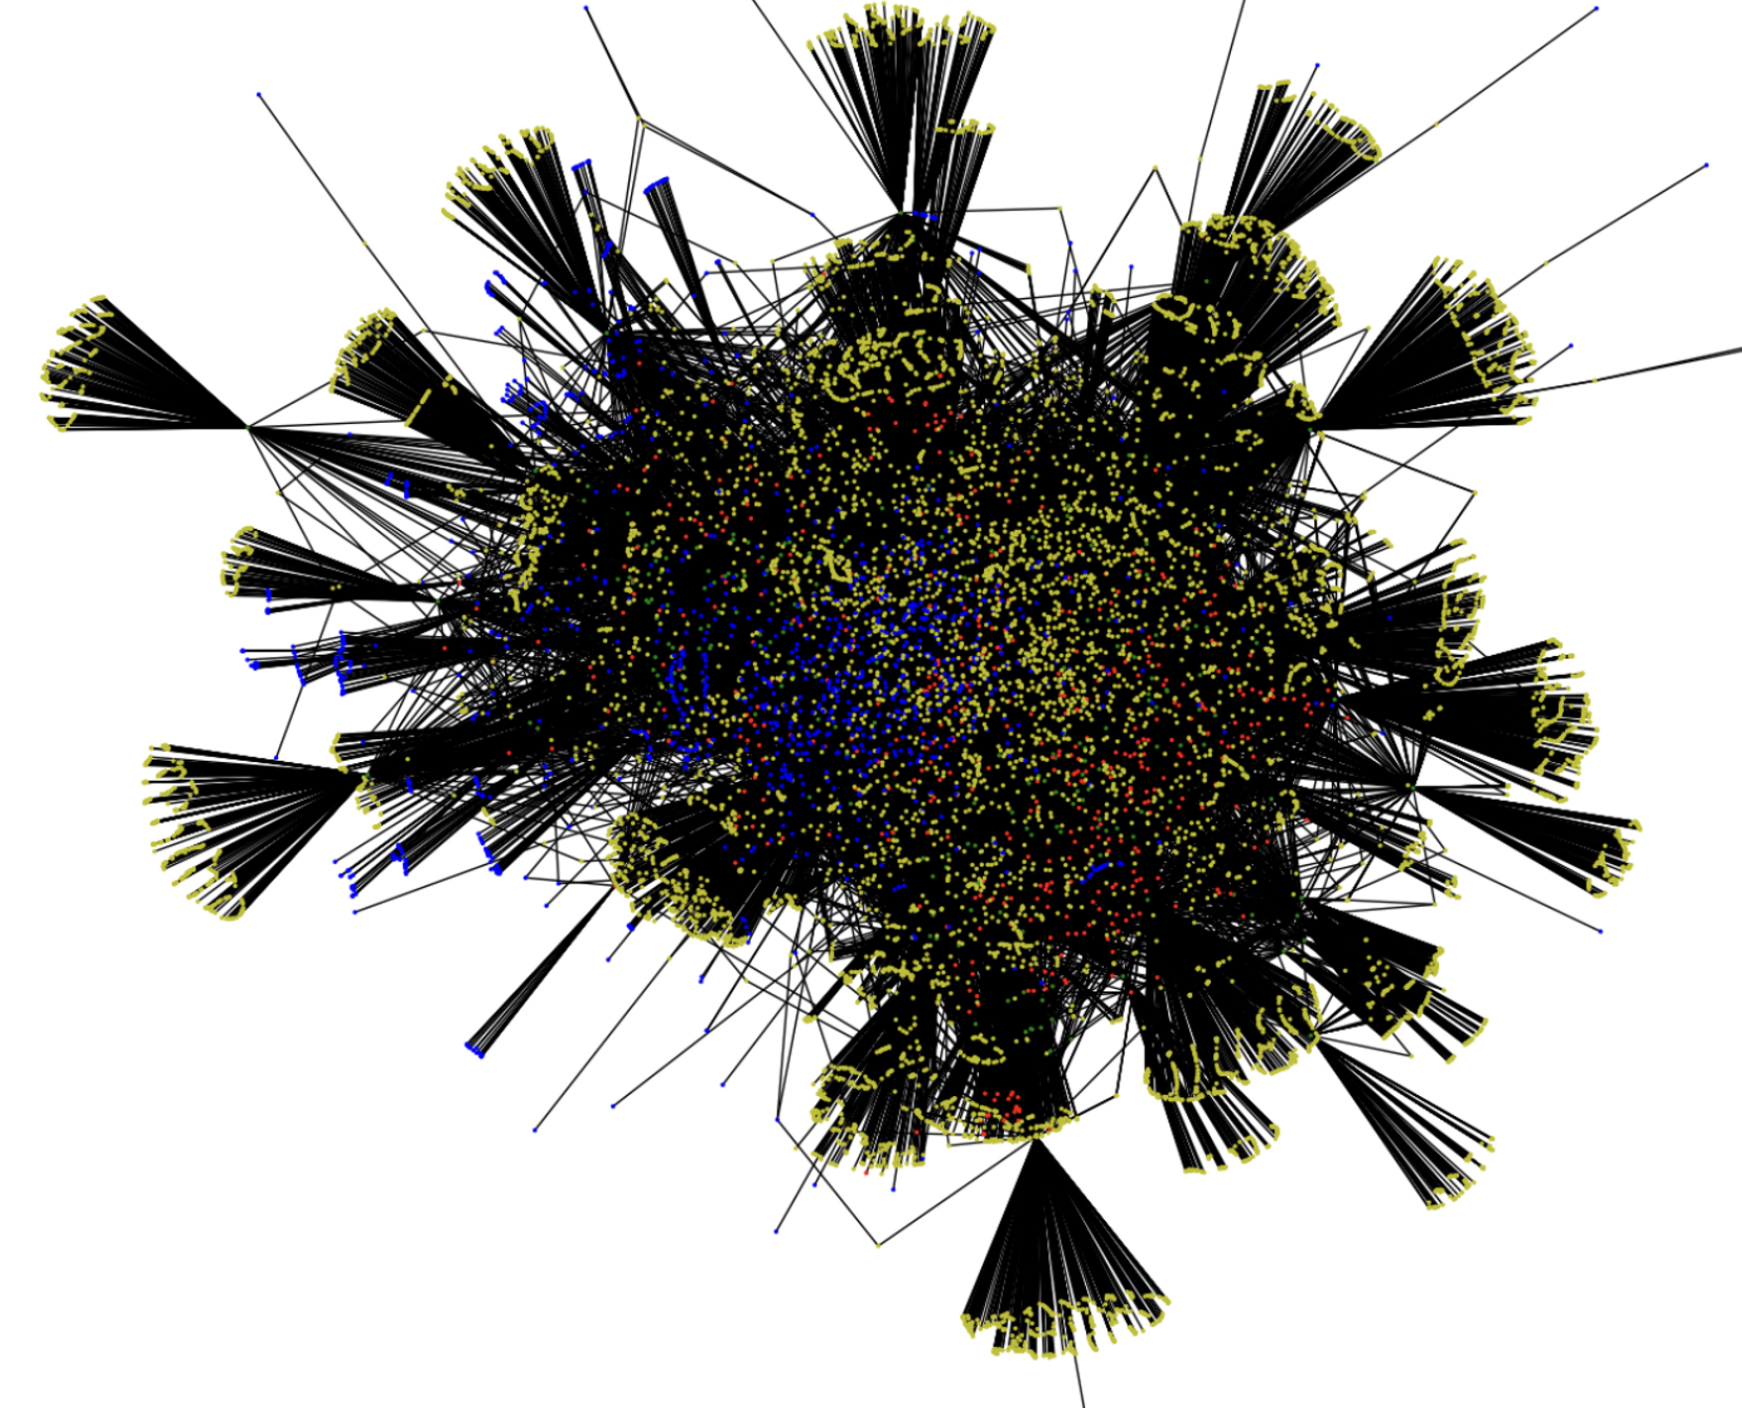
\includegraphics[scale=0.3]{./images/graph.png}
	\end{frame}

	\begin{frame}{GNNExplainer}
		GNNExplainer: Generating Explanations for Graph Neural Networks (Ying et al., 2019)
		$$
		\min _M-\sum_{c=1}^C \mathbf{1}[y=c] \log P_{\Phi}\left(Y=y \mid G=A_c \odot \sigma(M), X=X_c\right)
		$$
		\begin{itemize}
	\item If model predicts Ron Wyden traded Applied Materials Inc. (AMAT), then which nodes and edges are important for the prediction?
	\item Optimize node and edge masks $M$ that minimize the difference between prediction on the original graph and the masked graph.
	\item Can add L1 regularization to control the sparsity - how sparse (simple) explanation do you want?
	\item Aim to recover most simple but powerful explanation in form of subgraph of the original graph.
		\end{itemize}
	\end{frame}

	\begin{frame}{Ron Wyden - Applied Materials Inc. (AMAT)} 		
		\centering	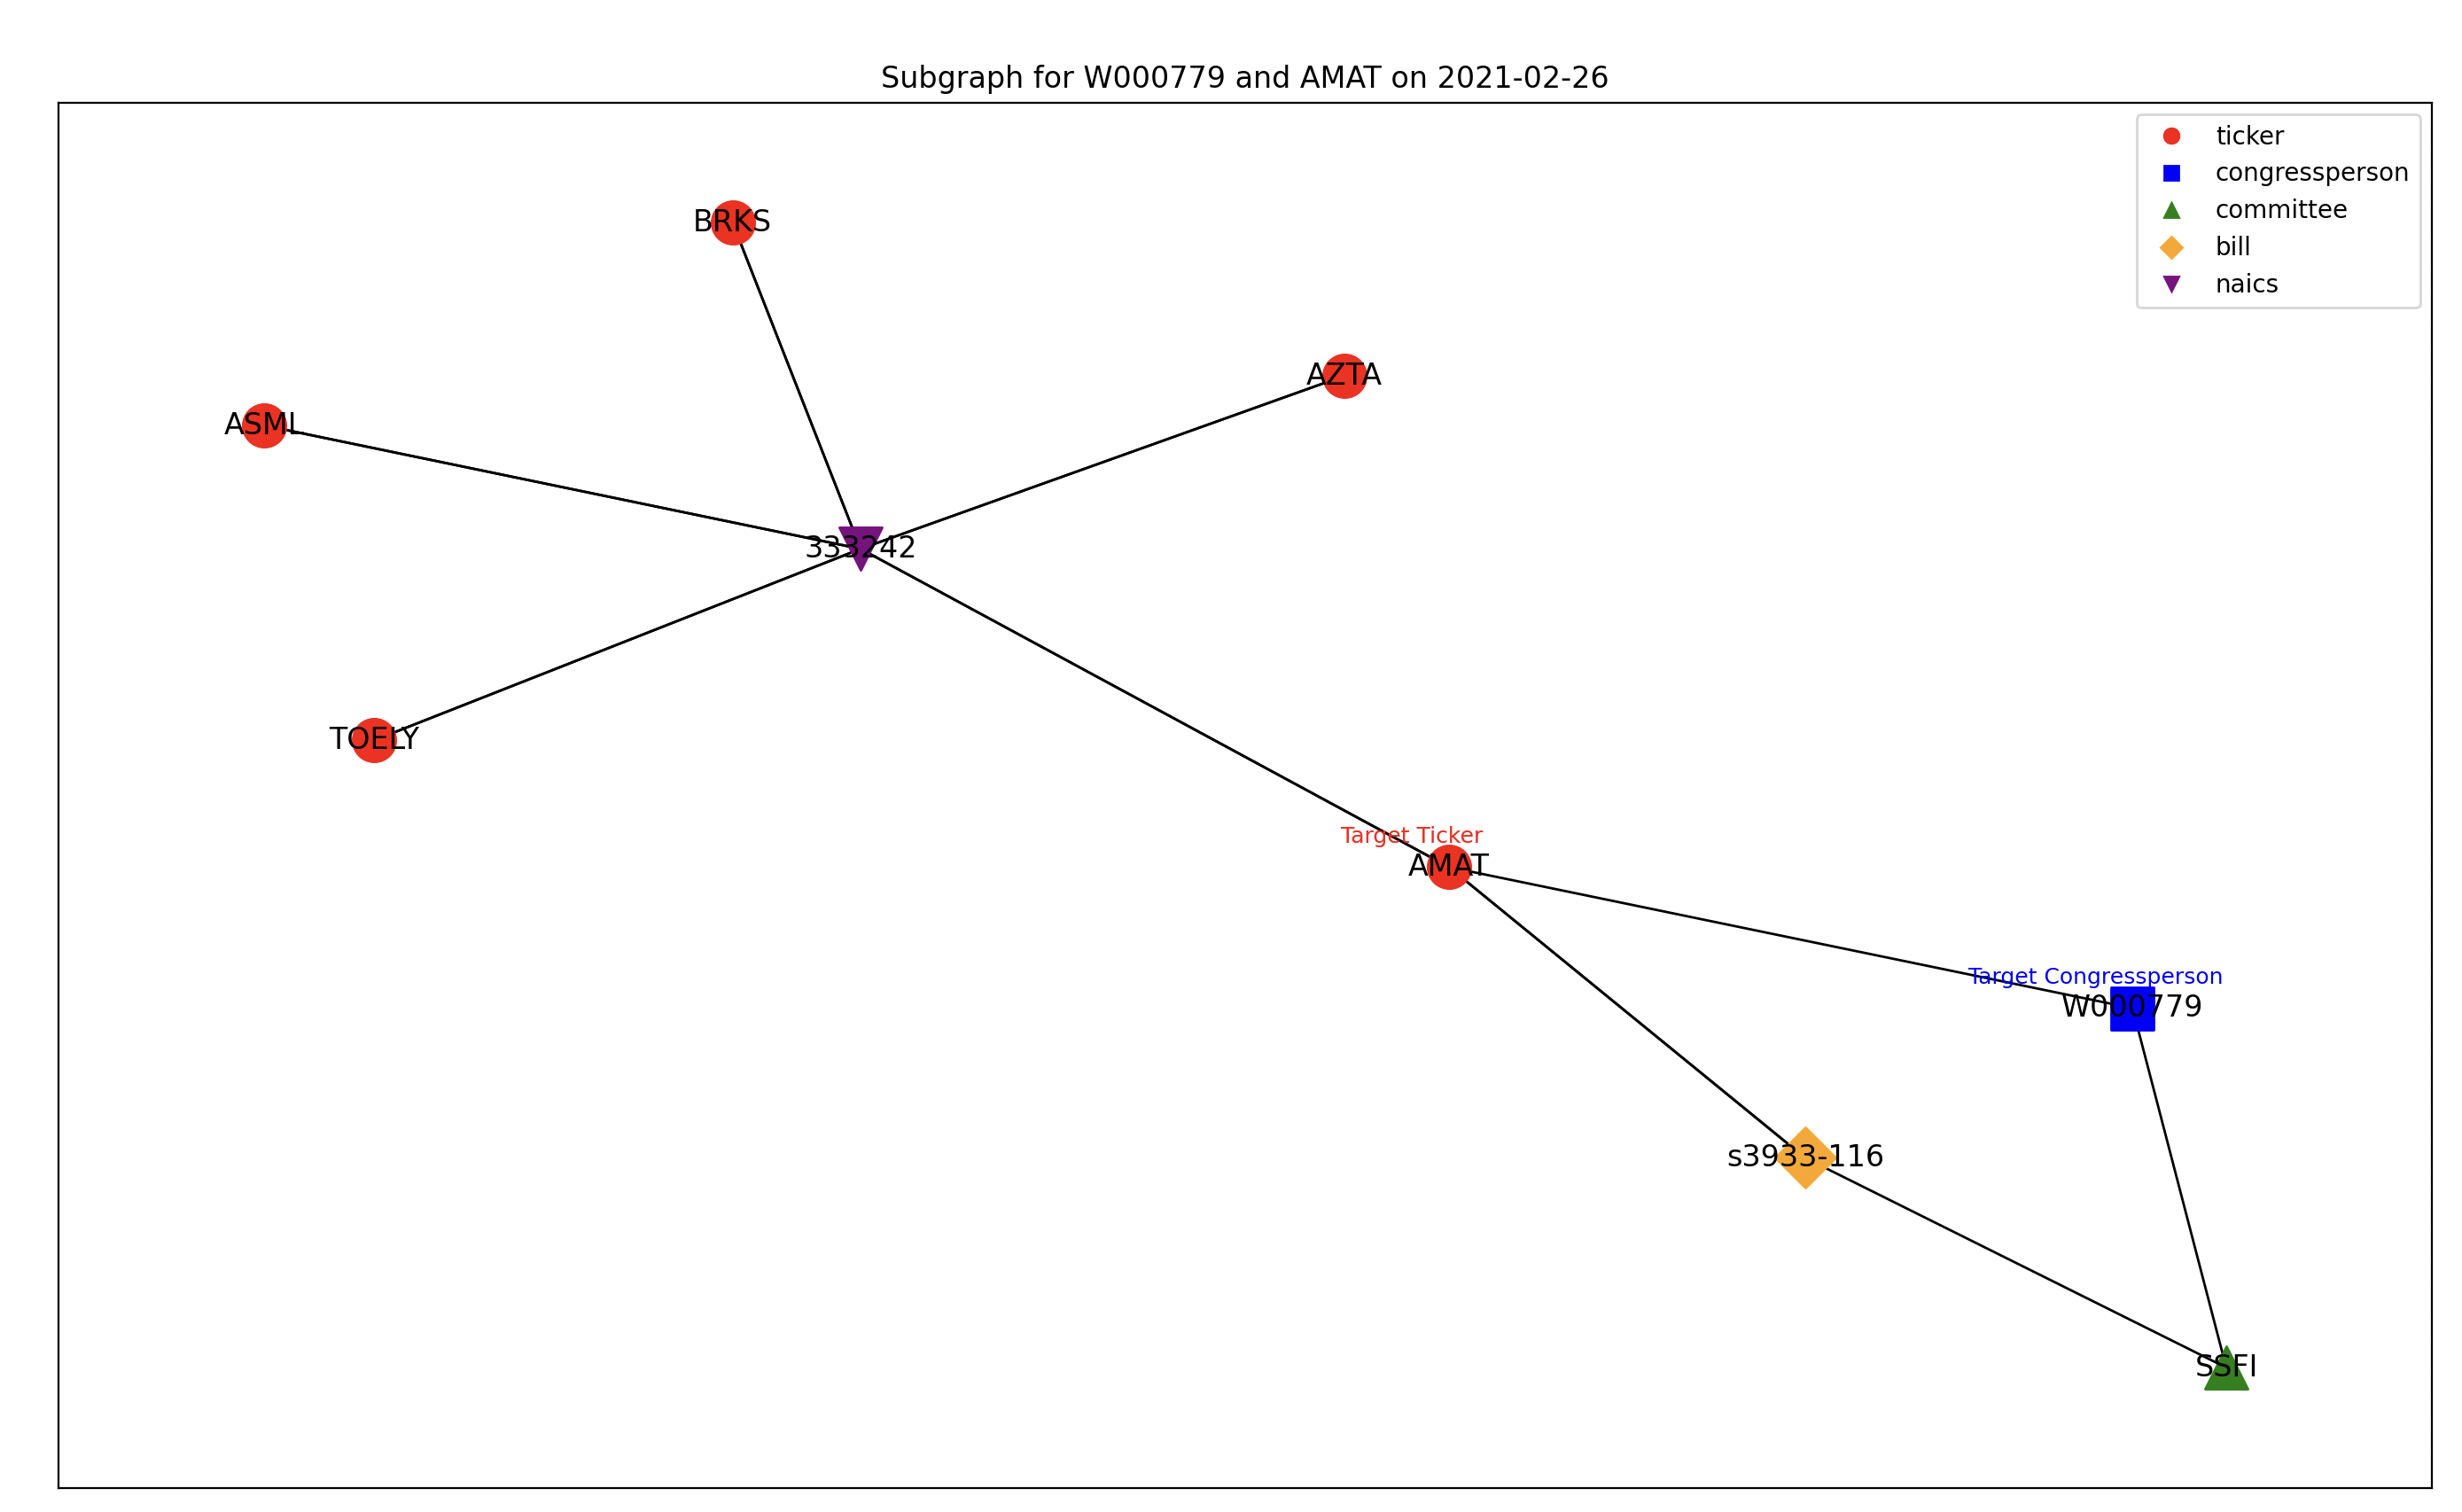
\includegraphics[scale=0.24]{./images/gnnex-w.png}
		\begin{itemize}
			\item S.3933-116: CHIPS ACT 
	\end{itemize}
	\end{frame}
	

	\begin{frame}{Dan Crenshaw - Rivian Automotive Inc (RIVN)} 		
		\centering	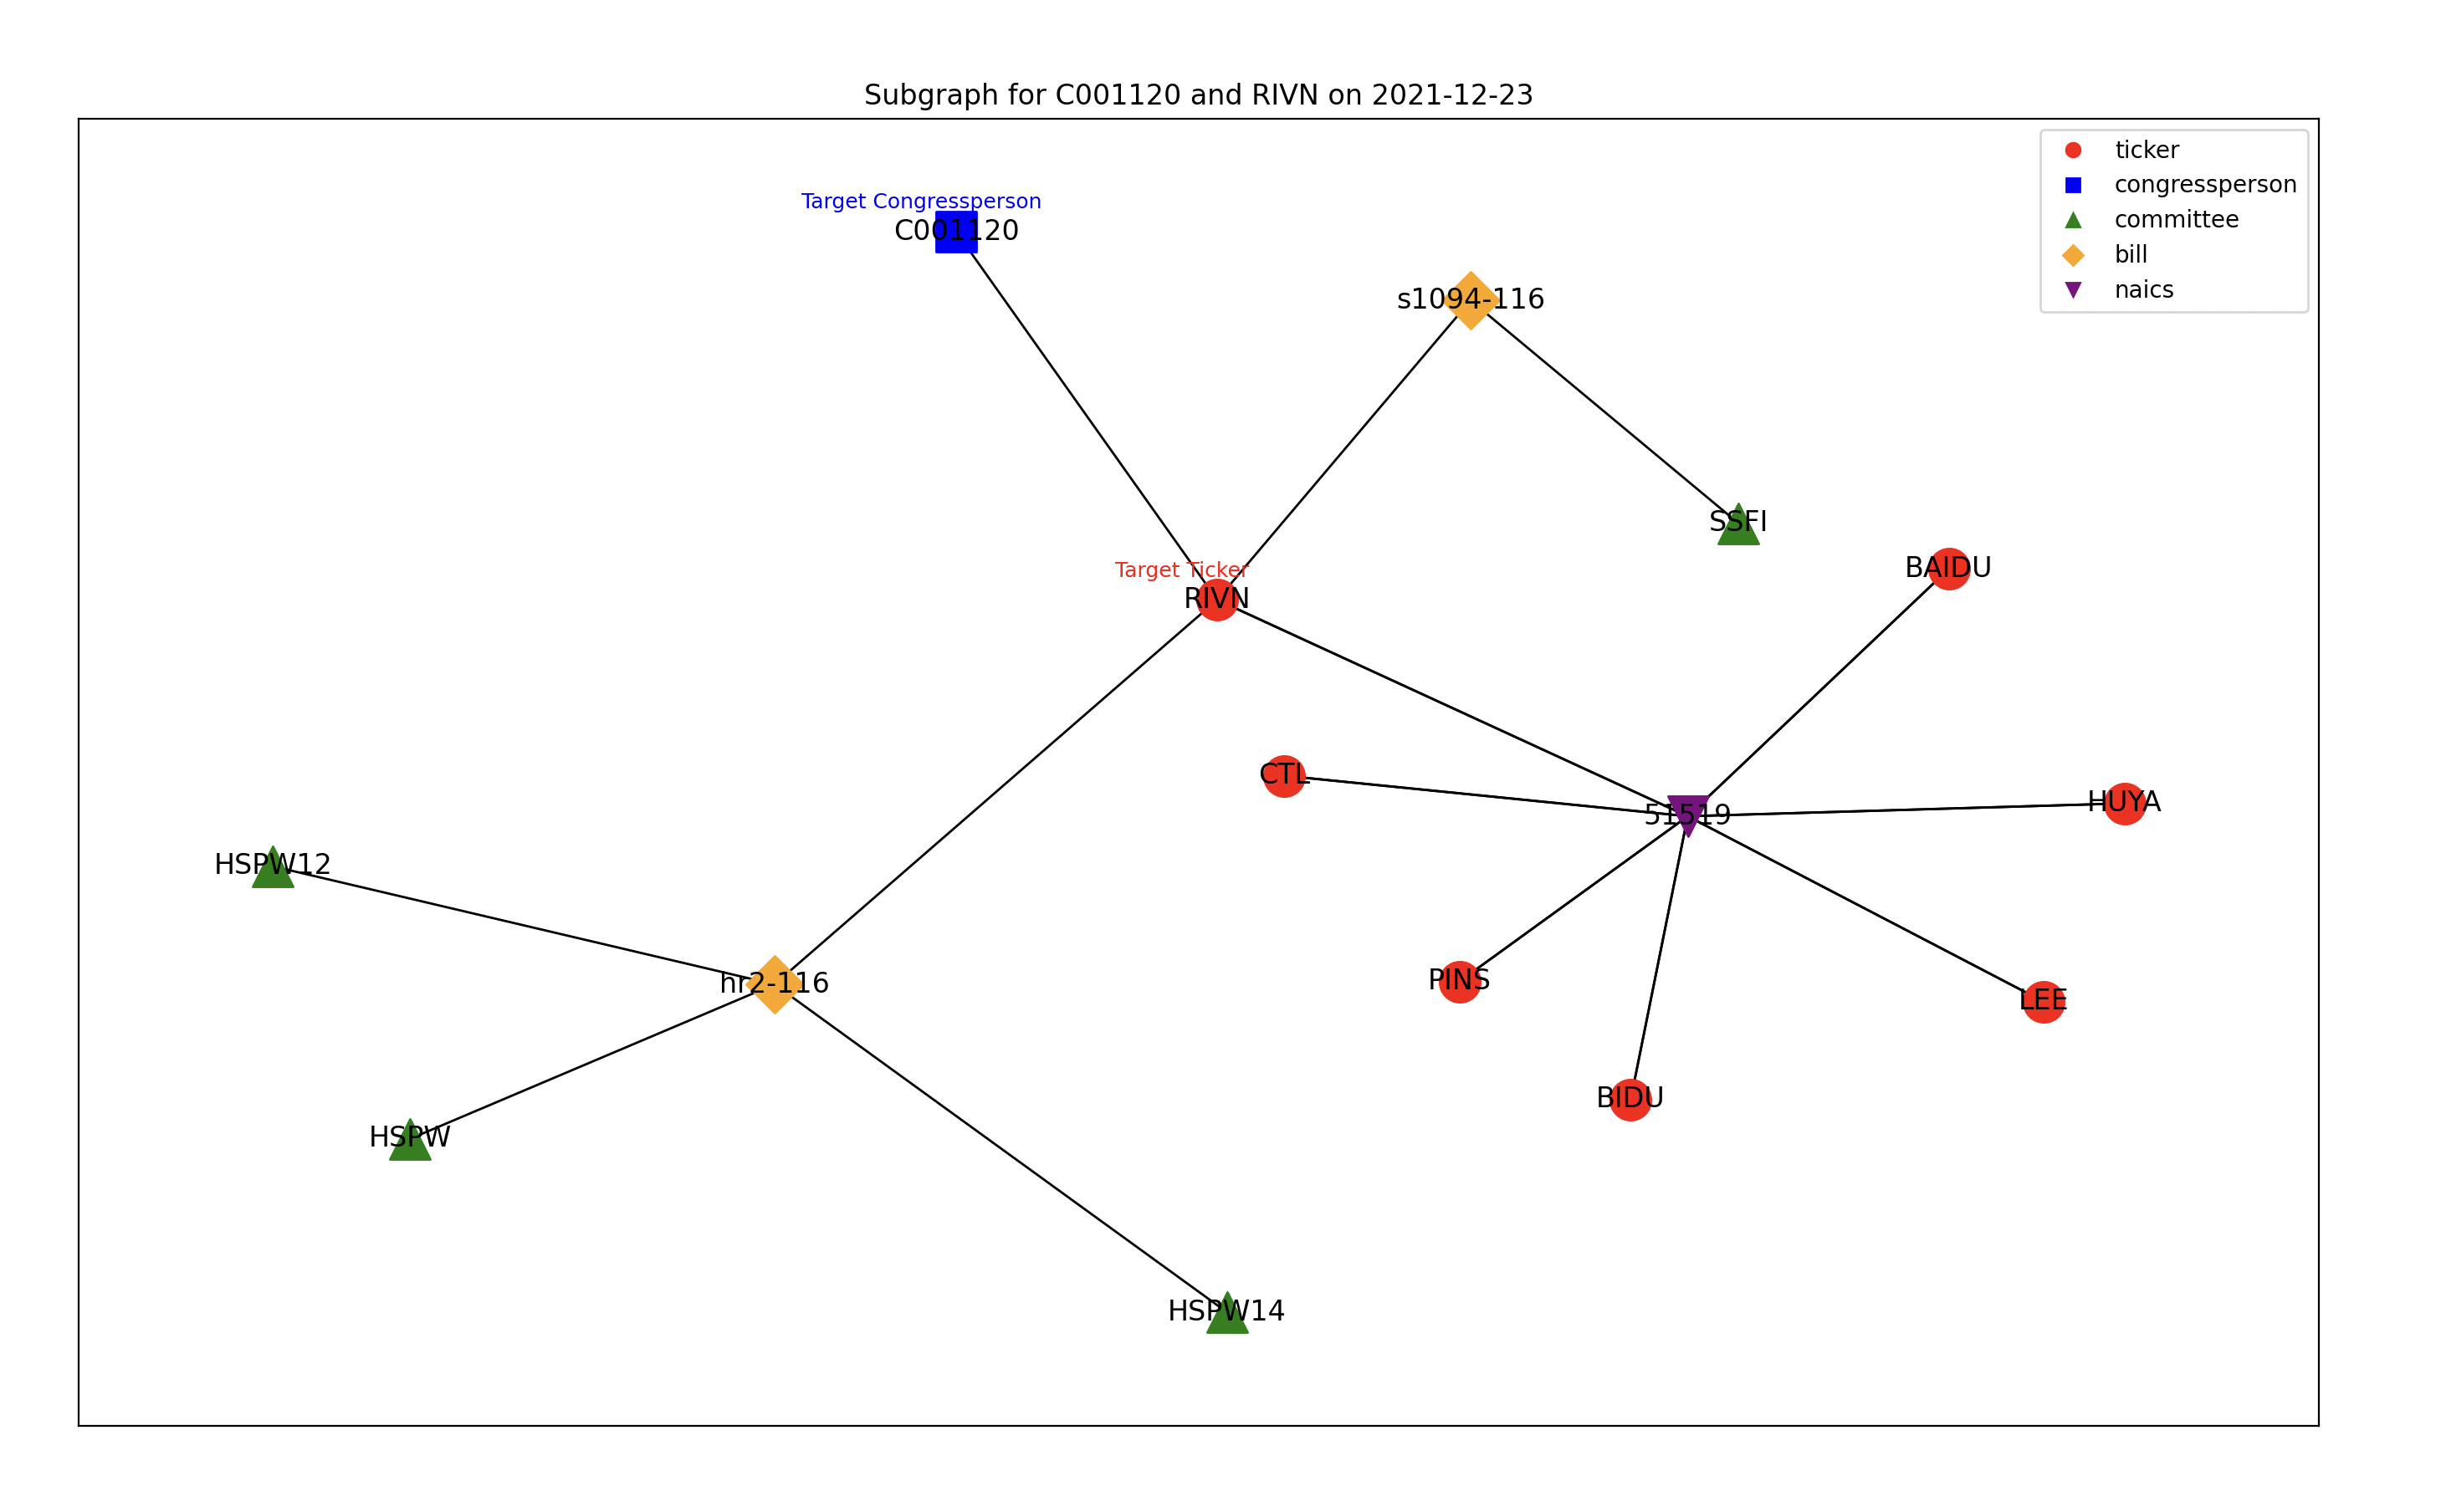
\includegraphics[scale=0.22]{./images/rvin.png}
		\begin{itemize}
			\item S.1094-116: Driving America Forward Act
	\end{itemize}
	\end{frame}

	\begin{frame}{Conclusion} 		
		\begin{itemize}
			\item Committee Assignments and Firm-level Lobbying on Bills are the most significant predictors of congresspersons' stock trading behavior, contrary to the findings of Egger and Hainmueller (2014).
			\item Congressional activities are informative for predicting congresspersons' stock trading.
			\item Future Research: Predict "excess returns" using the same graph data to assess the extent to which congressional activities can explain variations in excess returns.
		\end{itemize}
	\end{frame}
	
	

\end{document}

